\setchapterpreamble[u]{\margintoc}
\chapter{Մեկ փոփոխականի ֆունկցիա}
\labch{single_var}

\emergencystretch 2em

\section{Էքստրեմումի խնդիր}\label{apricot}

Պատկերացրեք՝ վեկտորների փոխարեն ունեք խանութ, և որոշակի հաշվարկների արդյունքում ստացել եք, որ խանութի եկամուտը ծիրանի գնից կախված է հետևյալ բանաձևով՝
\[
f(x) = 20\sqrt{x}-3x^3
\]
որտեղ $x$-ը $1$ կգ ծիրանի գինն է։

Ինչպես ցանկացած գործարար, Դուք ուզում եք հնարավորինս մեծացնել Ձեր եկամուտը, ուստի Ձեզ հետաքրքրում է հետևյալ հարցը․

\textit{— Որքա՞ն պետք է լինի $x$-ը, որպեսզի $f(x)$-ը լինի մաքսիմալ՝ հնարավորինս մեծ}

\question{\href{https://www.desmos.com}{\it Desmos} կամ \href{https://www.geogebra.org}{\it GeoGebra} ծրագրով գծեք $f(x)$-ի գրաֆիկը։ Ո՞րն է ծիրանի օպտիմալ գինը։}

Իրական կյանքում, իհարկե, իրավիճակն ավելի բարդ է, քանի որ ամեն խանութ ծիրանից բացի ուրիշ ապրանքներ էլ է վաճառում։ Եկամուտը կարող է կախված լինել մի քանի տարբեր գործոններից, օրինակ՝
\[
f(x,y,z,t) = 3xy^2-y\log t - (1-y) \log(1-t) + \frac{z^3}{t}
\]
որտեղ $x$, $y$, $z$, $t$-ի տվյալ պահին ունեցած արժեքներն են 
\[
x=4, \qquad y=0.4, \qquad z=0.8, \qquad t=55
\] 
և անհրաժեշտ է որոշել՝ մեծացնե՞լ, թե՞ փոքրացնել այդ արժեքները (և որքանո՞վ)։

Մեքենայական ուսուցման մեջ հաճախ նման անհայտները \marginnote{հաճախ այս խնդիրը անհնար է լու\-ծել․ փոխարենը որոնում են ոչ թե \textit{ամենա\-մեծ,} այլ \textit{համեմատաբար մեծ} արժեք} (պարա\-մետ\-րերը) ոչ թե մեկն են, այլ միլիոնից ավել, սակայն խնդիրը մնում է նույնը․ ինչպե՞ս գտնել տվյալ մեծության ամենամեծ կամ ամենափոքր արժեքը։ 

Նմանատիպ խնդիրները կոչվում են \textit{էքստրեմումի խնդիրներ,} և մենք կսկսենք մեր քննարկումը այն դեպքից, երբ ունենք միայն մի փոփոխական պարամետր։


\section{Հաջորդականություններ}

Սկսենք հաջորդականություններից։ \textit{Հաջորդականություն} ասելով՝ նկա\-տի կունենանք \textbf{անվերջ քանակով} թվերի՝ ֆիքսված հերթականու\-թյամբ գրված «շարք», «շարան»։

\begin{example}
Սրանք հաջորդականություններ են՝
\begin{itemize}
    \item $1,\; 2,\; 3,\; 4,\; 5,\; \dots$
    \item $1,\; -1,\; 1,\; -1,\; 1,\; \dots$
    \item $0,\; 0.2,\; 0.4,\; 0.6,\; 0.8,\; \dots$
    \item $6,\; 6,\; 6,\; 6,\; 6,\;  \dots$
\end{itemize}
իսկ սա՝ ոչ․
\begin{itemize}
    \item $1,\; 2,\; 3,\; 4$
\end{itemize}
\end{example}


Ինչ-որ իմաստով՝ հաջորդականությունը մեր իմացած վեկտորն է, բայց անվերջ երկարությամբ։ Ինչպես վեկտորները նշանակում ենք տառով՝
\[
\vv = \begin{bmatrix}
    v_1 \\ v_2 \\ \vdots \\ v_n
\end{bmatrix}
\]
իսկ նրա բաղադրիչները՝ նույն տառ + համարակալումով, այնպես էլ ամեն հաջորդականության կարող ենք տալ ինչ-որ անուն, ասենք՝ $a$, իսկ դրա \textit{անդամները} համարակալել՝
\[
a = (a_1,\, a_2,\, a_3,\, a_4,\, \dots )
\]

Քանի որ հաջորդականության բոլոր անդամները հերթով թվարկելն անհնար է (անվերջ հատ են), սովորաբար հարմարության համար պարզապես կգրենք, թե ի՞նչ բանաձևով է որոշվում դրա $n$-րդ ընդհանուր անդամը՝ $a_n$-ը։ 

Օրինակ՝ եթե ուզում ենք խոսել բնական թվերի քառակուսիներից բաղկացած հաջորդականության ($=$անվերջ չափանի վեկտորի) մասին, կգրենք՝
\[
a_n = n^2 \qquad \text{կամ} \qquad \{a_n\}=\{n^2\}
\]
և նկատի կունենանք, որ
\[
a_1 = 1, \qquad a_2 = 4, \qquad a_3 = 9, \qquad \dots 
\]
այսինքն՝ $a = (1,\, 4,\, 9,\, \dots)$:

\warning{Բազմություններում տարրերի հերթականությունը կարևոր չէ, մինչդեռ հաջորդականությունների դեպքում շատ կարևոր է․ $(1,\, 2,\, 3,\, 4,\, \dots) \ne (2,\, 1,\, 3,\, 4,\, \dots)$:}

Վեկտորների նմանությամբ կսահմանենք նաև հաջորդականությունների գումարը, տարբերությունը և թվով բազմապատկումը՝
\begin{align*}
(a_1,\, a_2,\, a_3,\, \dots) 
\pm
(b_1,\, b_2,\, b_3,\, \dots) 
&=
(a_1\pm b_1,\, a_2\pm b_2,\, a_3\pm b_3,\, \dots)% = a\pm b
\\
c \cdot 
(a_1,\, a_2,\, a_3,\, \dots) 
&=
(ca_1,\, ca_2,\, ca_3,\, \dots)% =c\cdot a
\end{align*}

Եթե բոլոր հաջորդականությունների բազմությունը նշանակենք $c$-ով, ապա $c$-ն կլինի գծային տարածություն (ինչպես վեկտորների բազմու\-թյունները)։ Ի տարբերություն վեկտորների՝ կսահմանենք նաև հաջոր\-դա\-կանությունների անդամ առ անդամ բազմապատկում և բաժանում՝
\begin{align*}
ab &= (a_1b_1,\, a_2b_2,\, a_3b_3,\, \dots) \\
\frac{a}{b}&=
\left(\frac{a_1}{b_1},\, \frac{a_2}{b_2},\, \frac{a_3}{b_3},\, \dots\right) \qquad \text{եթե $b_1, b_2, \dots \ne 0$}
\end{align*}

\question{Ի՞նչ հաջորդականությամբ բազմապատկենք $(1,\, 2,\, 3,\, 4,\, \dots)$ հաջորդականությունը, որպեսզի այն դառնա $(0,\, 0,\, 3,\, 0,\, 0,\, \dots)$:}

\section{Հաջորդականության սահման}

Կան հաջորդականությունների շատ հետաքրքիր օրինակներ։ Վերցնենք, օրինակ, հետևյալ հաջորդականությունը՝ $a_n = \dfrac{1}{n}$, այսինքն՝
\[
\left(1,\quad  \frac{1}{2},\quad \frac{1}{3},\quad \frac{1}{4},\quad \frac{1}{5},\quad \dots\right)
\]

Նկատենք, որ որքան $n$-ը մեծանում է, այնքան հաջորդականությունը փոքրանում ու փոքրանում է։ 

\begin{description}
    \item[Կա՞ այնպիսի թիվ, որին $\{a_n\}$-ը գնալով մոտենում է․] այո՛, որքան $n$-ը մեծանում է՝ $n\to\infty$, այնքան $a_n$-ը մոտենում է զրոյի՝ $a_n\to 0$։ Այս դեպքում $0$-ն կանվանենք $\{a_n\}$-ի \textit{սահման։}

    \item[Ինչ-որ պահի $a_n$-ը դառնո՞ւմ է $0$․] ո՛չ, հետաքրքիր է, սակայն որքան էլ հաջորդականության անդամները ձգտում են $0$-ին, մինևույն է՝ չեն հասնում, միշտ մնում են զրոյից մեծ։
\end{description}

\begin{definition}
Կասենք, որ  $\{a_n\}$ հաջորդականությունը \textbf{ձգտում} կամ \textbf{զուգամիտում} է $L$ թվին (կամ՝ $L$-ը $\{a_n\}$-ի \textbf{սահմանն} է), եթե $n$-ի բավարար մեծ արժեքների դեպքում բոլոր $a_n$ անդամները որքան ասես մոտ են լինում $L$-ին։

Դա կգրառենք այսպես՝
\marginnote{անգլերեն՝ {\it limit}, լատիներեն՝ {\it limes}}\[
\lim_{n\to\infty} a_n = L
\]
կամ այսպես՝
\[
a_n \to L \qquad (\text{երբ } n\to\infty)
\]
\end{definition}

Ի՞նչ նկատի ունենք, երբ ասում ենք՝ բնական թվերը անվերջ են։ Նկատի ունենք, որ ինչ թիվ էլ վերցնենք, գոյություն ունի այնպիսի բնական թիվ, որը դրանից ավելի մեծ է։ Նույն ձևով, երբ ասում ենք՝ $a_n \to L$, նկատի ունենք՝ ինչքան փոքր թիվ էլ վերցնենք (ասենք՝ $0.0001$) և հարցնենք՝ արդյո՞ք ինչ-որ պահի հաջորդականության բոլոր անդամները գտնվելու են $L$-ից ամենաշատը $0.0001$ հեռավորության վրա (այսինքն՝ շատ մոտիկ), պատասխանը լինելու է՝ \marginnote{այսինքն՝ կա ինչ-որ $N$ համար (ասենք՝ $N=2000$), որ դրանից հետո եկող բոլոր $n$-երի դեպքում՝ $|a_n-L|<0.0001$} այո, \textit{այսինչ պահից սկսած՝ բոլոր $a_n$-երը լինելու են $L$-ին $0.0001$ չափով մոտ։} 

\phantomsection \label{eps-delta}Ուստի կարող ենք $\lim\limits_{n\to\infty} a_n=L$ երևույթը ձևակերպել նաև այսպես՝
\begin{itemize}
 \item ինչ $\varepsilon>0$ թիվ էլ վերցնես
 \item գոյություն ունի բավարար մեծ $N$ թիվ այնպես, որ 
 \item $|a_n - L|<\varepsilon$ բոլոր $n=N,\ N+1,\ N+2,\ \dots$ անդամների համար
\end{itemize}

Նման ձևով կսահմանենք, որ $\lim\limits_{n\to\infty} a_n=+\infty$, եթե $a_n$-ը ցանկացած թվից մեծ է դառնում որոշ թվով քայլերից հետո։

\begin{definition}
Եթե $\{a_n\}$-ն ունի սահման, և այդ սահմանը վերջավոր է, ապա կասենք, որ այն \textbf{զուգամետ} է, հակառակ դեպքում՝ \textbf{տարամետ} է։
\end{definition}
    

\begin{example}
\\~
\begin{itemize}
    \item $1,\, 2,\, 3,\, 4,\, 5,\, \dots  \to +\infty$ 
    \item $1,\, -1,\, 1,\, -1,\, 1,\, \dots$ սահման չունի
    \item $0,\, 0.2,\, 0.4,\, 0.6,\, 0.8,\, \dots \to +\infty$
    \item $6,\, 6,\, 6,\, 6,\, 6,\,  \dots  \to 6$
\end{itemize}
\end{example}

\warning{Հաջորդականությունը կարող է ինչ-որ պահից սկսած հավասար լինել կամ չլինել իր սահմանին։}

Հաճախ կարելի է հաջորդականության բանաձևից որոշել նրա սահմանը․
\begin{itemize}
    \item $n^k \to \infty$ ցանկացած $k>0$ թվի համար
    \item $\dfrac{1}{n^k} \to 0$ ցանկացած $k>0$ թվի համար
    \item \marginnote{ի՞նչ կլինի, եթե $|c|=1$}$c^n\to +\infty$, եթե $c>1$, բայց $c^n \to 0$, եթե $|c|<1$
    \item եթե ինչ-որ պահից սկսած հաջորդականության բոլոր անդամները հավասար են նույն թվին, սահմանը այդ թիվն է 
\end{itemize}

\question{Ամեն ուրբաթ Ձեր տնօրենը կանչում է և ուրախությամբ հայտնում, որ Ձեր աշխատավարձը բարձրացվում է $0.99$ անգամ։ Քանի՞ շաբաթից կսկսեք զգալ, որ մի բան այն չէ։}

\begin{example}
\\~
\begin{itemize}
    \item $\lim\limits_{n \to \infty} \dfrac{1}{n} = 0$
    
    \item $\lim\limits_{n \to \infty} \left(\dfrac{2}{3}\right)^n  = 0$

    \item $\lim\limits_{n \to \infty} 0.3n  = \infty$ \; (տարամետ է)
\end{itemize}
\end{example}

Նկատենք նաև, որ երկու զուգամետ հաջորդականություններ գումարելիս, բազմապատկելիս, և այլ գործողություններ անելիս դրանց սահմանները պահպանվում են, այսինքն՝

\newpage
\begin{theorem}\label{limit_properties}
\\~
\begin{enumerate}
\item \marginnote{այստեղ $L$-ն ու $M$-ը \textbf{վերջավոր} թվեր են}Եթե $\lim\limits_{n \to \infty} a_n = L$ և $\lim\limits_{n \to \infty} b_n = M$, ապա
    \begin{align*}
        &\lim\limits_{n \to \infty} (a_n + b_n) = L + M\\
        &\lim\limits_{n \to \infty} (a_n - b_n) = L - M\\
        &\lim\limits_{n \to \infty} (a_n \cdot b_n) = L \cdot M\\
        &\lim\limits_{n \to \infty} \frac{a_n}{b_n} = \frac{L}{M} \qquad  \text{(եթե $M\ne0$)}
    \end{align*}
        
\item Եթե $\lim\limits_{n \to \infty} a_n = L$, ապա ցանկացած $c$ թվի համար
    \[
    \lim\limits_{n \to \infty} (c \cdot a_n) = c \cdot L
    \]
\begin{marginfigure}
    \caption*{$b$-ն սեղմված է $a$-ի ու $c$-ի արանքում, որոնք ձգտում են նույն $L$-ին}
    \centering
    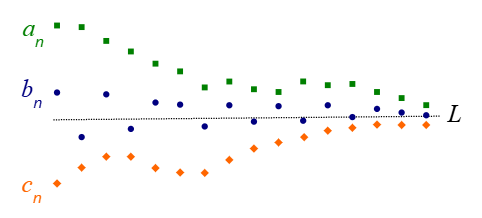
\includegraphics[width=\linewidth]{chapters/chapter 5/squeeze.png}
\end{marginfigure}
\item Եթե ցանկացած $n$-ի համար 
\[
a_n \leq b_n \leq c_n
\]
և $\lim\limits_{n \to \infty} a_n = \lim\limits_{n \to \infty} c_n = L$, ապա $\lim\limits_{n \to \infty} b_n = L$։
\end{enumerate} 
\end{theorem}

\question{Ենթադրենք $a_n \to 4$։ Ո՞ւր կձգտի հաջորդականությունը, եթե հեռացնեք նրա առաջին $3$ անդամները։}

Քանի որ ինչ-որ սահմանի ձգտելու համար անհրաժեշտ է, որ հաջորդա\-կանության անդամները \textit{սկսած ինչ-որ պահից} մոտ լինեն այդ սահմանին, նշանակում է՝ այդ սահմանը կախված չէ հաջորդականության առաջին $3$, $100$ կամ $1000$ անդամներից։ Եթե ի վերջո հաջորդականու\-թյու\-նը մոտենում է ինչ-որ թվի, ապա սկզբի մի քանի անդամներ\marginnote{թեև, իհարկե, ամեն բան կարող է փոխվել, եթե ջնջեք կամ ավելացնեք \textit{անվերջ թվով} անդամներ} փոխելիս, ջնջելիս կամ ավելացնելիս այդ զուգամիտությունը չի փոխ\-վում։

\section{Ֆունկցիայի սահման}

\question{Ի՞նչ եք կարծում, ի՞նչ է նշանակում $\lim\limits_{x\to 0} \left(2+x\right)^3$ արտա\-հայտու\-թյունը։}

Ինչպես հաջորդականությունների համար $n$-ը ձգտեցնելով անվերջի և մոտենալով ինչ-որ թվի՝ այն անվանեցինք սահման, այդպես էլ ներմուծենք սահմանի գաղափարը ֆունկցիաների համար։ 

Վերցնենք օրինակ՝
\[
f(x) = \left(2+x\right)^3
\]
ֆունկցիան։ Ո՞ր մեծությունը կուզեինք անվանել $f(x)$-ի սահման $x=0$ կետում։ Ինտուիտիցիան մեզ հուշում է, որ եթե գծեինք $f(x)$-ի գրաֆիկը և նայեինք, թե $x$-ը $0$-ին մոտենալիս ի՞նչ թվի է մոտենում $f(x)$-ի արժեքը, հենց այդ թիվն էլ պետք է որ համարել \textit{$f$-ի սահմանը $0$ կետում։}

Այլ կերպ ասած՝ եթե $0$-ի ձգտող ինչ $\{x_n\}$ հաջորդականություն էլ վերցնենք ու տեղադրենք $f$-ի մեջ, և արդյունքում ստացվող $\left(f(x_1),\, f(x_2),\, f(x_3),\, \dots\right)$ հաջորդականությունը ձգտի ինչ-որ թվի, սահմանը կլինի այդ թիվը։ Ուրեմն սահմանենք $a \in \R$ կետում $f$-ի սահմանը․

\begin{definition}
Եթե \textbf{ցանկացած} $x_n\to a$ հաջորդականության համար
\[
f(x_1), \;\; f(x_2), \;\; f(x_3), \;\; \dots,\;\;f(x_n),\;\;\dots
\]
հաջորդականությունը ձգտում է միևնույն $L$ թվին, ապա $L$-ը կոչվում է $f$ ֆունկցիայի \textbf{սահման $a$ կետում՝}
\[
\lim\limits_{x\to a} f(x) = L
\]
\end{definition}

\begin{figure}[t]
    \centering
    \subfloat{{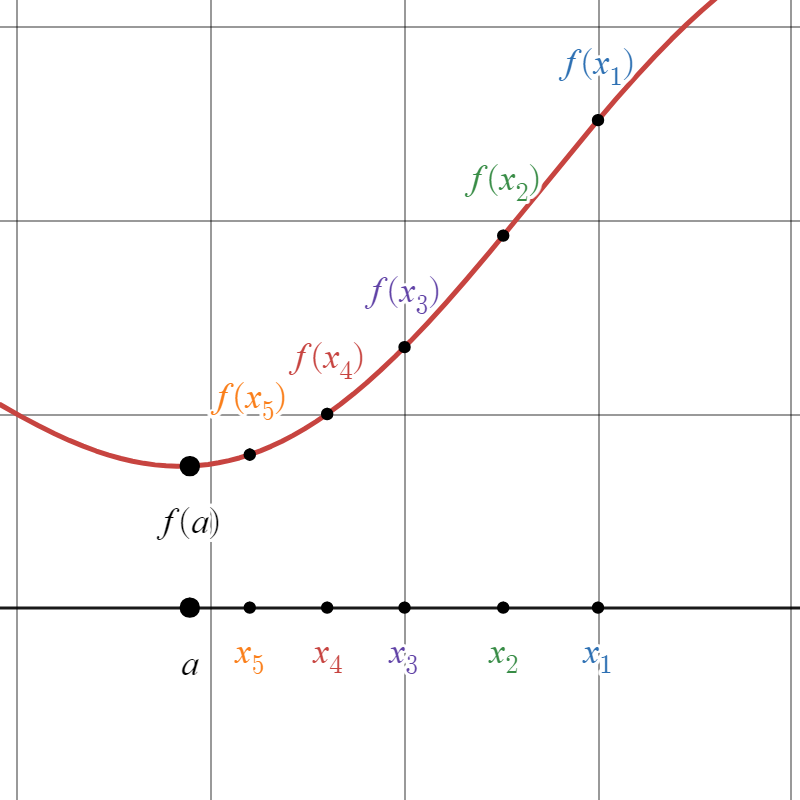
\includegraphics[width=0.4\linewidth]{chapters/chapter 5/cont limit.png} }}%
    \qquad
    \subfloat{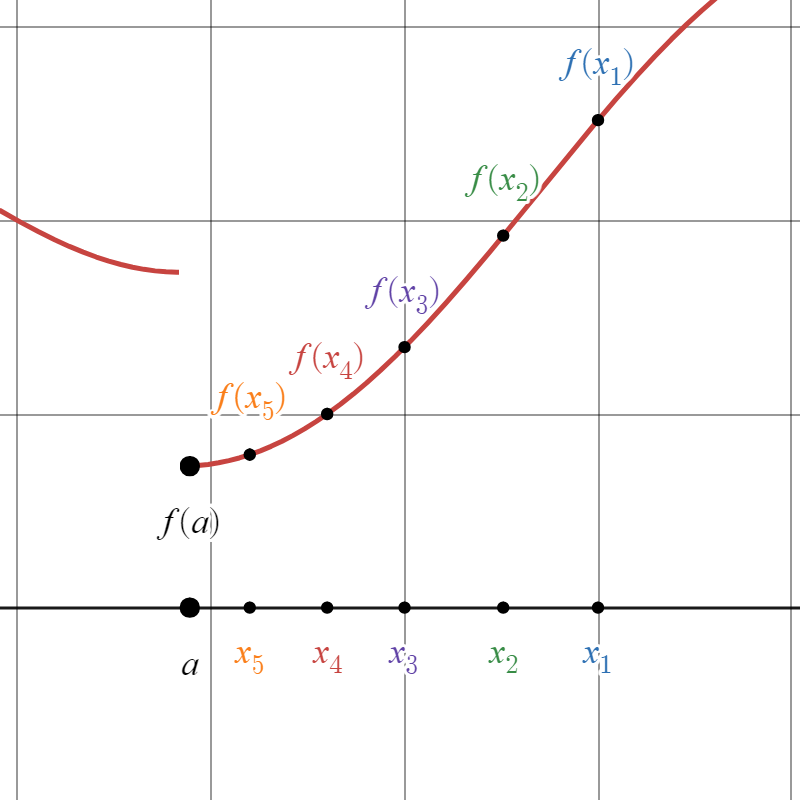
\includegraphics[width=0.4\linewidth]{chapters/chapter 5/disc limit.png}} %
    \caption*{ձախ նկարի ֆունկցիան $a$ կետում ունի սահման, իսկ աջինը՝ չունի, քանի որ եթե $x_n$-երը վերցնեինք $a$-ից ձախ, $f(x_n)$-ը կմոտենար մի ուրիշ թվի}
\end{figure}

Ինչո՞ւ ենք նշում «\textit{ցանկացած} $x_n \to a$-ի համար»։ Բանն այն է, որ երբեմն որոշ ֆունկցիաներ իրենց այնքան էլ լավ չեն պահում․ երբ $a$-ին մոտենում ենք աջից, ստանում ենք ինչ-որ սահման, բայց երբ մոտենում ենք ձախից՝ ստանում ենք մեկ այլ սահման։ Նման դեպքերում կասենք, որ ֆունկցիան $a$ կետում սահման չունի։

\warning{Ֆունկցիան կարող է մի կետում ունենալ սահման, մի ուրիշ կետում՝ ոչ։}

Կրկին ինչպես \hyperref[eps-delta]{\color{OliveGreen}հաջորդականությունների դեպքում}, սահմանը կարող ենք սահմանել նաև այսպես․ կասենք, որ $\lim\limits_{x\to a}f(x)=L$, եթե \marginnote{ինչքան էլ փոքր $\varepsilon$ ասես՝ եթե $x$-ը $a$-ին բավարար մոտ լինի, ապա $f(x)$-ը մոտ կլինի $L$-ին (ոչ հեռու, քան $\varepsilon$ չափով)} ցանկացած $\varepsilon>0$ թվի համար գոյություն ունի այնպիսի $\delta>0$ թիվ, որ եթե $0<|x-a|<\delta$, ապա $|f(x)-L| < \varepsilon$:

\begin{example}
\\~
\begin{itemize}
    \item $\lim\limits_{x \to 0}(2+x)^3 = 2^3 = 8$
    \item $\lim\limits_{x \to 4}(2+x)^3 = 6^3 = 216$
    \item $\lim\limits_{x \to -3}(2+x)^3 = (-1)^3 = -1$
    \item $\lim\limits_{x \to 2.5}4x-3 = 4\cdot 2.5-3 = 7$
    \item $\lim\limits_{x \to 9}\sqrt{x} = \sqrt{9} = 3$
    \item $\lim\limits_{x \to 0}e^x = e^0 = 1$
\end{itemize}
\end{example}

Ինչպես տեսնում ենք, հաճախ տրված կետում սահմանը հաշվելու համար պետք է ընդամենը այդ կետը տեղադրել ֆունկցիայի մեջ և վերջ։

\begin{figure}[h]
    \centering
    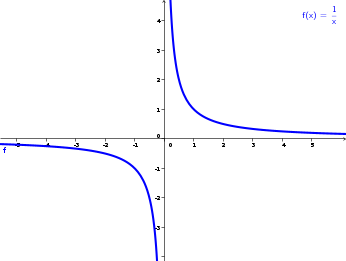
\includegraphics[width=0.65\linewidth]{chapters/chapter 5/1 over x.png}
\end{figure}

Օրինակ՝ $f(x) = \dfrac{1}{x}$ ֆունկցիայի գրաֆիկից երևում է, որ երբ $x$-ը մոտեցնում ենք $3$ կետին, ֆունկցիայի ընդունած արժեքները մոտենում են $\dfrac{1}{3}$-ին, հետևաբար՝ $\lim\limits_{x \to 3} \dfrac{1}{x}=\dfrac{1}{3}$:

Իսկ ի՞նչ կարող ենք ասել $0$ կետում սահմանի մասին։ Եթե $x$-ը $0$ կետին մոտեցնենք աջից, $f(x)$-ի արժեքները աճելով կձգտեն $+\infty$-ի, մինչդեռ եթե ձախից մոտենանք՝ կձգտեն $-\infty$-ի։ Սա նշանակում է, որ ֆունկցիան $0$ կետում սահման չունի։ Ավելին, եթե $x=3$-ում ֆունկցիան որոշված է՝ \marginnote{$f$-ը կարծես երկու իրար հետ կապ չունեցող ֆունկցիա լինի}ունի արժեք, ապա $x=0$-ում ֆունկցիան արժեք էլ չունի՝ որոշված չէ։ Նման դեպքում կասենք, որ $f$-ը $0$ կետում \textit{խզվող} է, իսկ մնացած կետերում՝ \textit{անընդհատ։}

\begin{definition}
Կասենք, որ $f$ ֆունկցիան \textbf{անընդհատ} է $a$ կետում, եթե
\begin{enumerate}
    \item $f$-ը $a$-ում որոշված է\marginnote{ունի արժեք}
    \item $\lim\limits_{x \to a} f(x)$ սահմանը գոյություն ունի\marginnote{ունի սահման}
    \item $\lim\limits_{x \to a} f(x) = f(a)$\marginnote{արժեք $=$ սահման}
\end{enumerate}
\end{definition}

Պատկերավոր ասած՝ տվյալ կետում ֆունկցիան անընդհատ է, եթե դրա գրաֆիկը հնարավոր է գծել՝ առանց գրիչը թղթից կտրելու։

\warning{Ֆունկցիան կարող է մի կետում անընդհատ լինել, մի ուրիշ կետում՝ խզվել։}

Անընդհատությունը շատ օգտակար հատկություն է, և գործնականում հանդիպող ֆունկցիաները, բարեբախտաբար, մեծ մասամբ անընդհատ են $(-\infty, \infty)$ ընկած բոլոր կետերում (ողջ $\R$-ում), կամ մեկ-երկու կետից բացի մնացած բոլոր կետերում,\marginnote{օրինակ՝ $\sqrt{x}$-ը կամ $\dfrac{1}{x}$-ը, որոնք ոչ բոլոր կետերում են որոշված} կամ էլ՝ բոլոր այն կետերում, որտեղ որոշված են։ 

Նշենք, որ եթե որևէ $a$ կետում $f$-ն ու $g$-ն անընդհատ են, ապա դրանք գումարելիս, հանելիս, բազմապատկելիս, բաժանելիս կամ թվով բազմապատկելիս ստացվող ֆունկցիաները՝
\begin{itemize}
    \item $f+g$
    \item $f-g$
    \item $f\cdot g$
    \item $\dfrac{f}{g}$ (եթե $g(a) \ne 0$)
    \item $cf$ ($c$-ն ցանկացած թիվ է)
\end{itemize}
նույնպես անընդհատ են այդ կետում։

\question{Կռահո՞ւմ եք, թե ինչպիսի տարածություն է կազմում $a$ կետում անընդհատ բոլոր ֆունկցիաների բազմությունը։}


\begin{figure}[t]
\centering %
\floatsetup{floatrowsep=qquad}
\begin{floatrow}[3]%
\ffigbox[\FBwidth]{\caption*{\centering անընդհատ\linebreak (բոլոր կետերում որոշված)}}{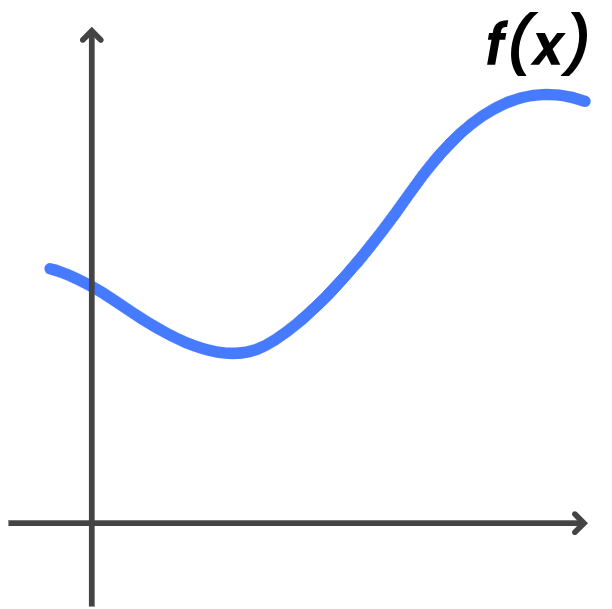
\includegraphics[width=0.4\textwidth]{chapters/chapter 5/continuity 1.png}}
\ffigbox[\FBwidth]{\caption*{\centering խզվող\linebreak (բոլոր կետերում որոշված)}}{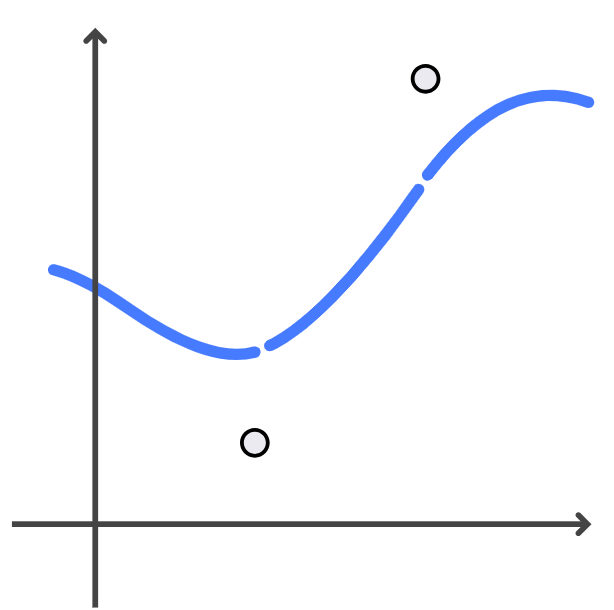
\includegraphics[width=0.4\textwidth]{chapters/chapter 5/continuity 2.png}}
\ffigbox[\FBwidth]{\caption*{\centering խզվող\linebreak (ոչ բոլոր կետերում որոշված)}}{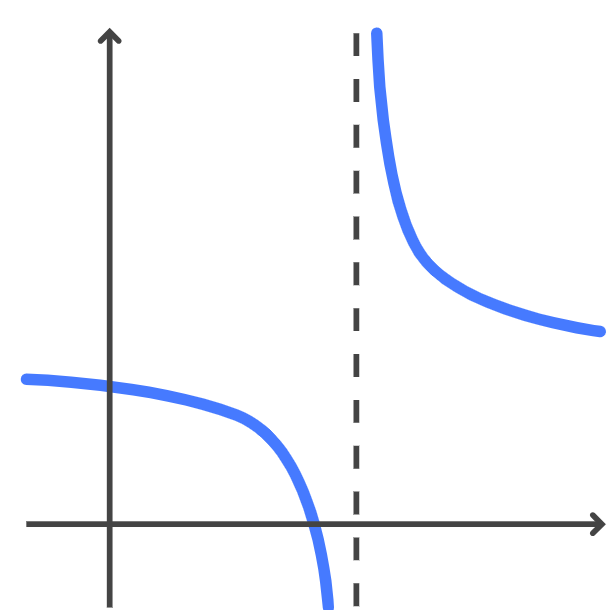
\includegraphics[width=0.4\textwidth]{chapters/chapter 5/continuity 3.png}}
\end{floatrow}
\end{figure}

Եթե ֆունկցիան բոլոր կետերում անընդհատ է (կամ գոնե՝ բոլոր այն կետերում, որոնցում որոշված է), ապա այն կարճ կասենք ուղղակի \textit{անընդհատ ֆունկցիա։} Անընդհատ ֆունկցիաներ են, օրինակ՝
\begin{itemize}
    \item հաստատուն ֆունկցիաները՝ $3$, $-8$
    \item գծային ֆունկցիաները՝ $3x+4$, $5x$, $y-x$
    \item առհասարակ բոլոր բազմանդամները՝ $x^2+7x-1$, $xy-y^4+z$
    \item արմատ պարունակող ֆունկցիաները՝ $\sqrt{x}$, $\sqrt[5]{x}$
    \item ցուցչային ու լոգարիթմական ֆունկցիաները՝\marginnote{որոշները ոչ բոլոր կետերում են որոշված} $2^x$, $e^{3x}$, $\ln{x}$
    \item եռանկյունաչափական ֆունկցիաներն ու դրանց հակադարձները՝ $\cos(3x)$, $\arcsin{x}$
\end{itemize}
և այլն։ Խզվող ֆունկցիաները հեշտ է պարզել՝ նայելով դրանց գրաֆիկին։ Եթե ինչ-որ կետի մոտենալիս ֆունկցիայի արժեքը տարբեր կողմերից տարբեր թվերի է ձգտում, կամ ասենք՝ գրաֆիկը մի որևէ կետում կտրվում է, ապա ֆունկցիան խզվող է։


\section{Ածանցյալ}

Պատկերացրեք՝ փոքրացել-դարձել եք կետ և ֆունկցիայի գրաֆիկի վրայով կարուսելի նման սահում եք վերև ու ներքև։ Ձեր ճանապարհը ֆունկցիայի գրաֆիկն է․ ինչ-որ ժամանակ դրանով կբարձրանաք դեպի վեր, հետո կսկսեք իջնել, հետո նորից բարձրանալ, երբեմն՝ ավելի մեծ արագությամբ կընթանաք, երբեմն՝ շարժումը կդանդաղի։

\begin{figure}[h]\label{local_extr}
    \centering
    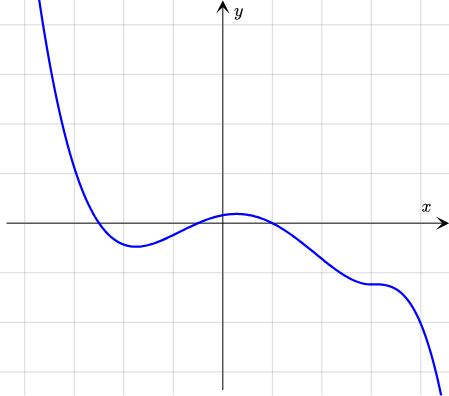
\includegraphics[width=0.6\linewidth]{chapters/chapter 5/just function.png}
\end{figure}

Բայց փաստացի՝ հիմա Դուք կետ չեք։ Գրաֆիկով մեկ սահել չեք կարող, փոխարենը պետք է բավարարվեք ֆունկցիայի բանաձևով։ Ինչպե՞ս կարող ենք բանաձևից ելնելով՝ պարզել, թե երբ ու ինչպես են տեղի ունենում ֆունկցիայի այս վայրիվերումները։

Նախ ֆիքսենք, թե գրաֆիկի ո՞ր կետում եք գտնվում, և փորձենք հաշվել այդ կետում Ձեր ունեցած արագությունը։ Ենթադրենք՝ գտնվում ենք ${x=a}$ \marginnote{ֆունկցիայի ընդունած արժեքը՝ $f(a)$} կետում։

\question{Ինչպե՞ս կհաշվեք, թե տնից խանութ գնալու ճանապարհին որքա՞ն է Ձեր մոտավոր արագությունը։}

Եթե այժմ $a$ կետից մի փոքր շարժվենք դեպի աջ կամ ձախ, ասենք՝ շատ չնչին $h$ չափով\marginnote{եթե ձախ ենք շարժվում, $h$-ը կվերցնենք բացասական}, ապա կհայտնվենք $f(a+h)$-ում, այսինքն՝ $h$ չափով քայլ կատարելու դեպքում կբարձրանանք/կիջնենք 
\[
f(a+h) - f(a)
\]
չափով։ Եթե հիմա այս փոփոխության չափը բաժանենք մեր կատարած քայլի վրա՝
\[
\frac{f(a+h) - f(a)}{h}
\]
կստանանք «միջին» կամ «միավոր» փոփոխության չափը ($a$ կետի շուրջն այս ու այն կողմ գնալիս)։

Վերջապես, քանի որ ուզում ենք չափել հենց $a$ կետում մեր շարժման արագությունը,\marginnote{$a$-ից հեռու $f$-ի արագությունը կարող է ավելի մեծ/փոքր լինել, բայց դա $a$-ում արագության վրա չպետք է ազդի} ապա պետք է կենտրոնանանք միայն $a$ կետին շատ մոտիկ շրջակայքի վրա։ Այլ կերպ ասած՝ ստիպենք, որ $h$-ը լինի շա՜տ փոքր՝
\[
\lim_{h\to 0} \frac{f(a+h) - f(a)}{h}
\]

Ինչ թիվ որ արդյունքում ստանանք, հենց դա էլ ցույց կտա $a$-ում մեր (այսինքն՝ $f$-ի գրաֆիկի աճել/նվազելու) արագությունը։ Այդ թիվը կոչվում է $a$ կետում $f$-ի \textit{ածանցյալ։}

\begin{definition}
Եթե հետևյալ սահմանը գոյություն ունի և անվերջ չէ՝\marginnote{կամ որ նույնն է՝ $\displaystyle \lim_{{x\to a}} \frac{f(x) - f(a)}{x-a}$}
\[
\lim_{h \to 0} \frac{f(a + h) - f(a)}{h}
\]
ապա այն կնշանակենք $f'(a)$-ով կամ $\dfrac{df}{dx}(a)$-ով և կանվանենք $f$ ֆունկցիայի \textbf{ածանցյալ} $a$ կետում։
\end{definition}

Եթե $f$-ն $a$-ում ունի ածանցյալ, ապա կասենք, որ այն \textit{ածանցելի} կամ \textit{դիֆերենցելի} է $a$ կետում։

\begin{example}
Դիտարկենք $f(x) = x^2$ ֆունկցիան։ Որևէ $x$ կետում դրա ածանցյալը հաշվելու համար գրենք՝
\[
f'(x) = \lim\limits_{{h \to 0}} \frac{(x + h)^2 - x^2}{h} =  \lim\limits_{{h \to 0}} \frac{x^2+2xh+h^2 - x^2}{h} = 2x
\]
Ուրեմն՝ ցանկացած $x$ կետում $f$-ի ածանցյալն է՝ $f'(x) = 2x$։
\end{example}

Եվս մեկ անգամ արձանագրենք, որ ֆունկցիայի ածանցյալը տվյալ կետում ցույց է տալիս այդ ֆունկցիայի \textit{փոփոխման արագությունը՝} որքան է փոխվում ֆունկցիայի արժեքը,\marginnote{որքան զգայուն է ֆունկցիան իր արգու\-մեն\-տի փոփոխության նկատմամբ} երբ նրա արգումենտը մի փոքր փոփոխում ենք։ Իհարկե, ֆունկցիան կարող է երբեմն արագանալ, երբեմն՝ դանդաղել, հետևաբար՝

\warning{Ածանցյալը տարբեր կետերում ընդունում է տարբեր ար\-ժեքներ․ $f'(x)$-ը ոչ թե ֆիքսված թիվ է, այլ $x$-ից կախված ֆունկցիա։}
\question{Որքան $x$-ը գնում է աջ, այնքան $f(x)=x^2$-ու ածանցյալը մեծանում է։ $f$-ի գրաֆիկին նայելով՝ ինչպե՞ս կմեկնաբանեք դա։}
Նշենք, որ եթե անընդհատությունը լավ հատկություն է, ապա դիֆերեն\-ցելիությունը էլ ավելի լավ հատկություն է։ Մասնավորապես,

\begin{theorem}
Եթե ֆունկցիան որևէ կետում դիֆերենցելի է, ապա նաև անընդհատ է այդ կետում։
\end{theorem}

Բայց հակառակը ճիշտ չէ․ կան ֆունկցիաներ, որոնք անընդհատ են, բայց դիֆերենցելի չեն։

\begin{example}
\begin{marginfigure}
    \centering
    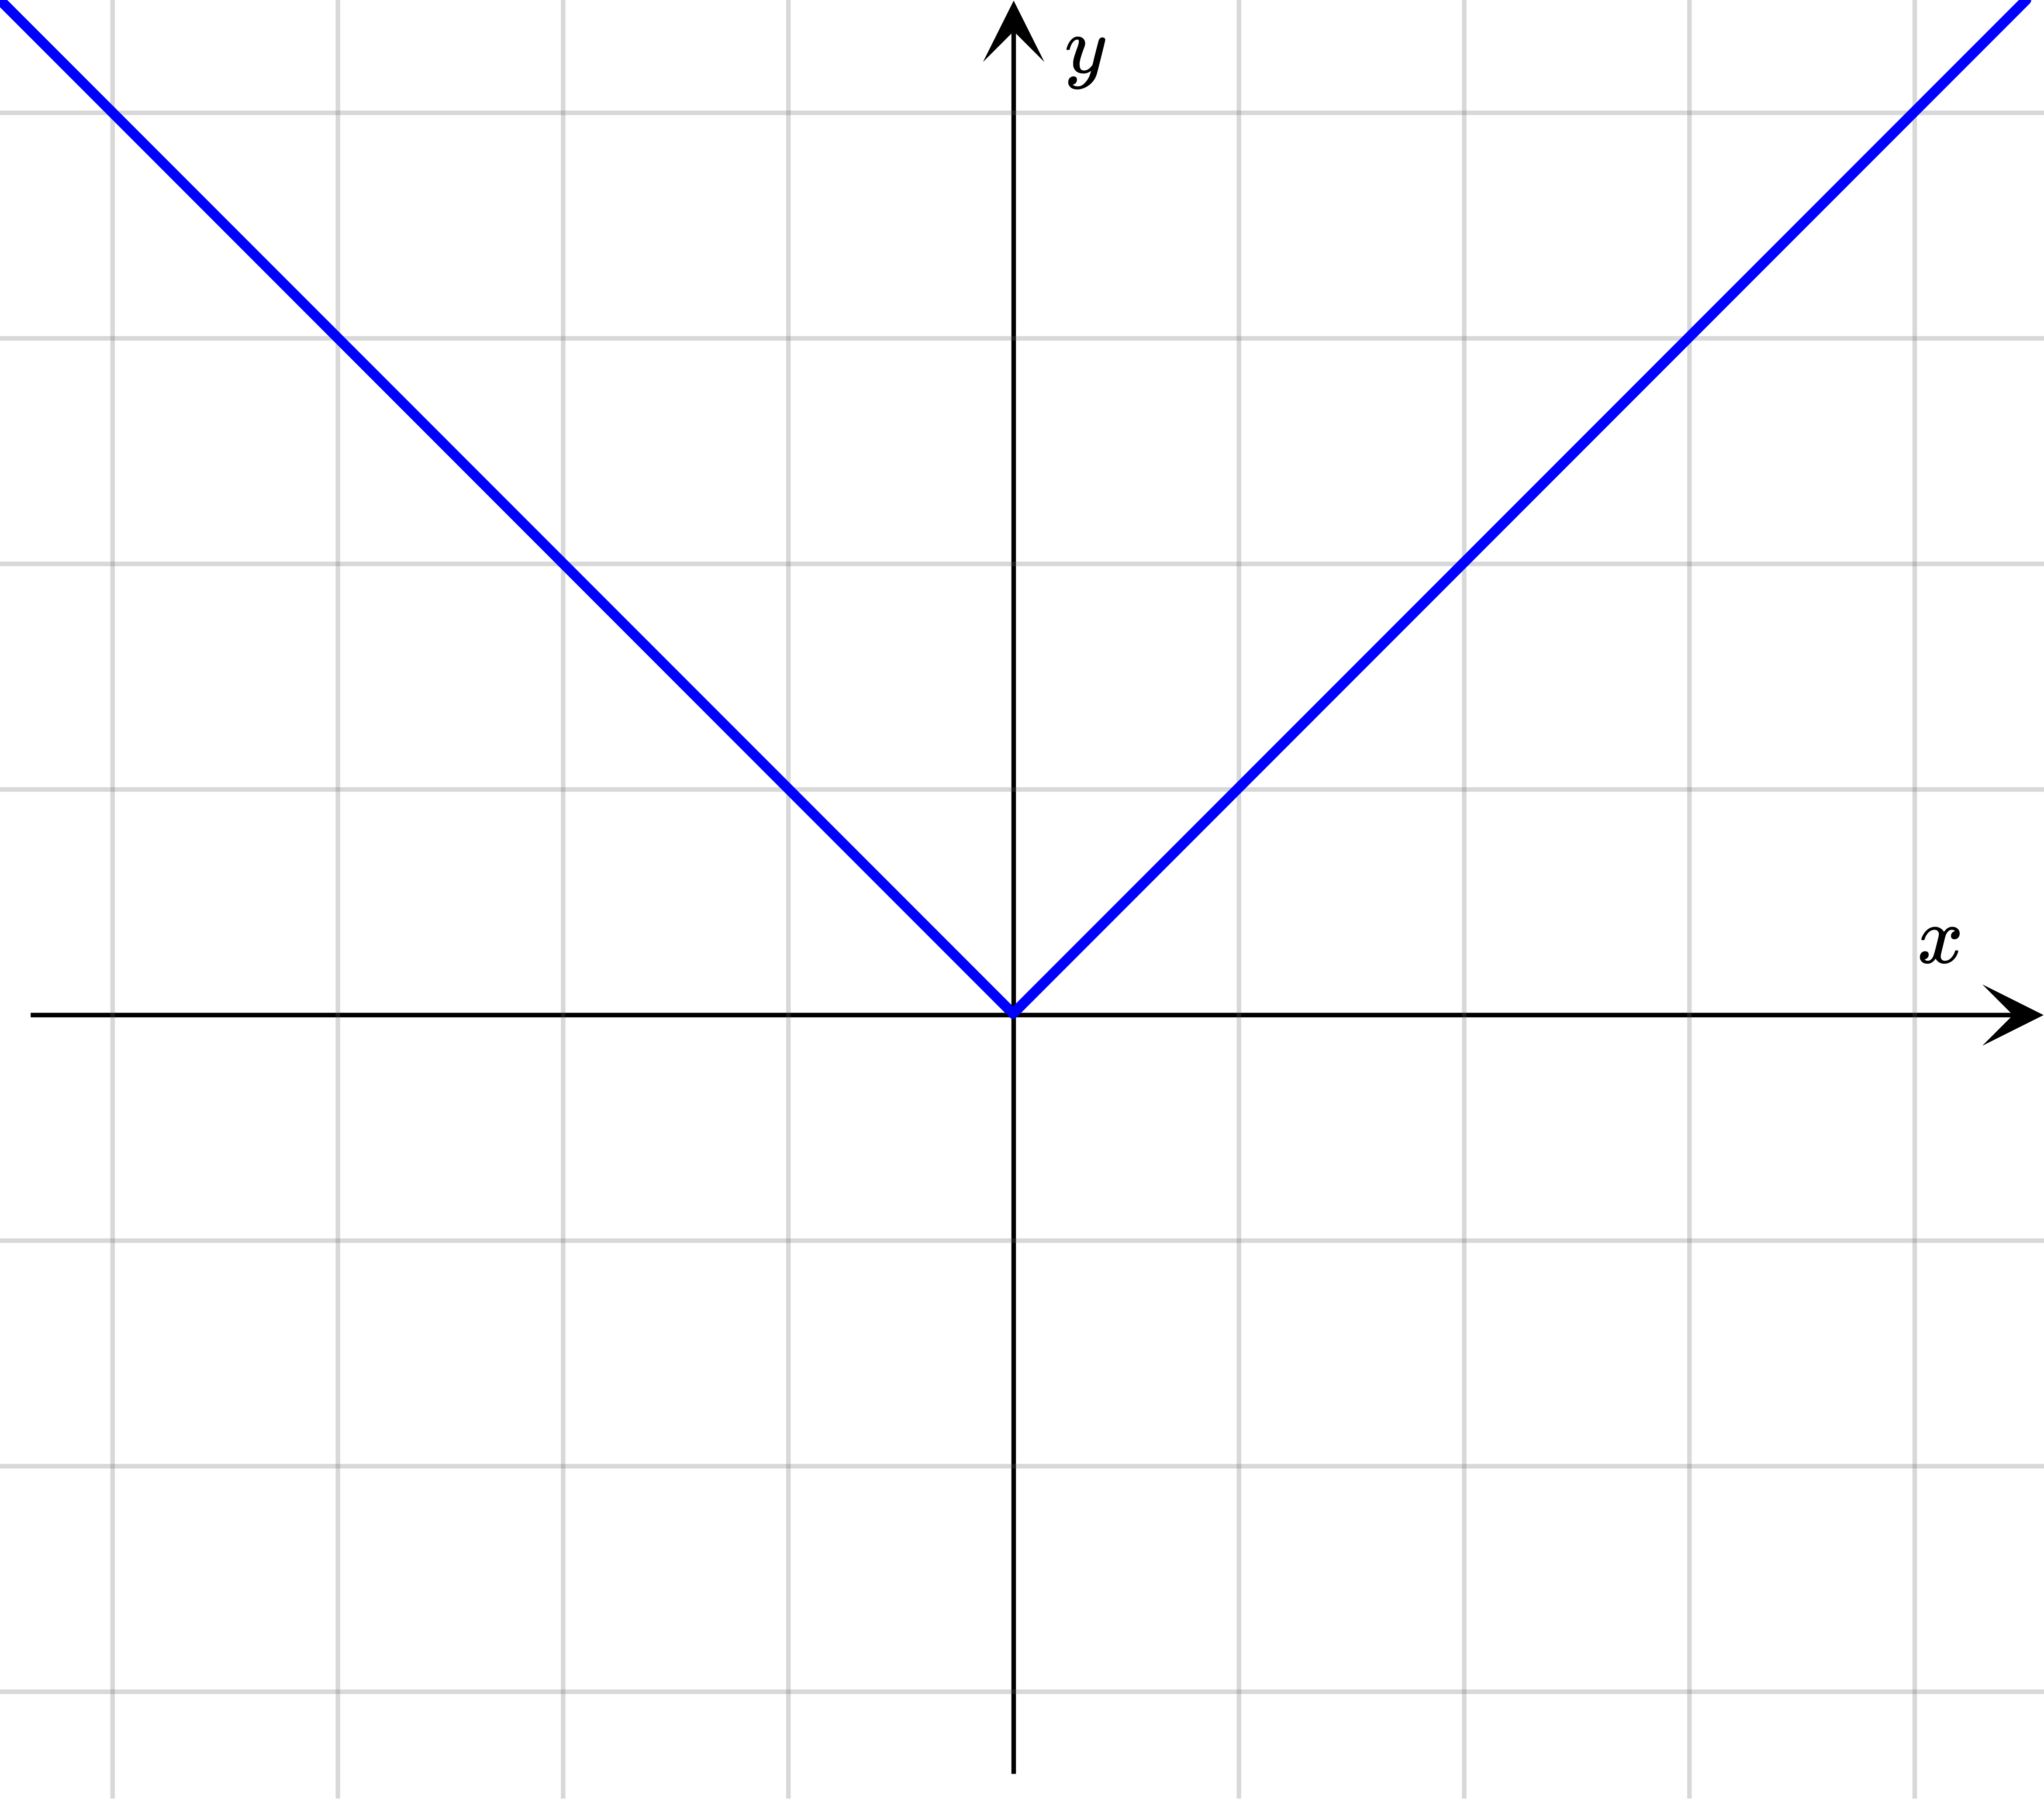
\includegraphics[width=1\linewidth]{chapters/chapter 5/abs(x).png}
    \caption*{կարծես երկու ֆունկցիաներ $0$ կետում կպցրած լինեն միմյանց, բայց ոչ այնքան սահուն ձևով}
\end{marginfigure}
$f(x)=|x|$ ֆունկցիան անընդհատ է, նրա ածանցյալը դրական $x$-երում $1$ է՝
\[
\lim_{h\to 0} \frac{|x+h|-|x|}{h}
=
\lim_{h\to 0} \frac{x+h-x}{h}
=
1
\]
բացասական կետերում՝ $-1$՝
\[
\lim_{h\to 0} \frac{|x+h|-|x|}{h}
=
\lim_{h\to 0} \frac{-(x+h)-x}{h}
=
-1
\]
Իսկ այ $x=0$ կետում ֆունկցիան ածանցյալ չունի, քանի որ եթե $0$-ին մոտենանք 

\begin{itemize}
    \item \item աջից՝ $h>0$, կունենանք՝ $\dfrac{|0+h|-|0|}{h}=\dfrac{h}{h}=1$
    \item ձախից՝ $h<0$, կունենանք՝ $\dfrac{|0+h|-|0|}{h}=\dfrac{-h}{h}=-1$
\end{itemize}

Ընդհանուր դեպքում $h$-ը $0$-ի ձգտելիս սահման չկա, հետևաբար $f$-ը $0$-ում դիֆերենցելի չէ։
\end{example}

Ինչպես կարող եք ենթադրել՝ նայելով գրաֆիկին, ածանցյալ չունենալու պատճառը $0$ կետում ուղղության շատ կտրուկ փոփոխությունն է։

\question{Որքա՞ն կլինի $f(x)=14$ հաստատուն ֆունկցիայի ածանցյալը։}

Նման եղանակով կարող ենք հաշվել մի քանի հաճախ հանդիպող ֆունկցիաների ածանցյալները․ \phantomsection \label{derivatives_list}
\begin{itemize}
    \item $(c)' = 0$ \marginnote[*+1]{հաստատունի ածանցյալը $ = 0$}
    \item $(x)' = 1$
    \item $(x^2)' = 2x$
    \item $(x^n)' = nx^{n-1}$ 
    % \marginnote{մասնավորապես՝\\$\left(\dfrac{1}{x}\right)'=\left(x^{-1}\right)'=-x^{-2}=-\dfrac{1}{x^2}$\\$\left(\sqrt{x}\right)'=\left(x^{1/2}\right)'=\dfrac{1}{2}x^{-1/2}=\dfrac{1}{2\sqrt{x}}$}
    \item $(e^x)' = e^x$
    \item $(a^x)' = a^x\ln a$
    \item $(\ln x)' = \dfrac{1}{x}$
    \item $(\sin x)'=\cos x$
    \item $(\cos x)'=-\sin x$
\end{itemize}
իսկ չորրորդ կանոնից մասնավորապես հետևում է, որ
\begin{itemize}
    \item $\left(\dfrac{1}{x}\right)'=\left(x^{-1}\right)'=-x^{-2}=-\dfrac{1}{x^2}$
    \item $\left(\sqrt{x}\right)'=\left(x^{1/2}\right)'=\dfrac{1}{2}x^{-1/2}=\dfrac{1}{2\sqrt{x}}$
\end{itemize}

\question{Ի՞նչ եք կարծում, որքա՞ն է $e^x + \cos x$-ի ածանցյալը։}

Արդեն հայտնի ֆունկցիաներից բաղկացած այլ ֆունկցիաների ածանց\-յալը հաշվելիս օգտակար են հետևյալ բանաձևերը․
\begin{itemize}
    \item $(cf)'=c\cdot f'$
    \item $(f + g)'=f' + g'$
    \item $(f - g)'=f' - g'$
    \item $(fg)'=f'g+fg'$
    \item $\left(\dfrac{1}{f}\right)'=-\dfrac{f'}{f^2}$ (եթե $f\ne 0$)
    \item $\left(\dfrac{f}{g}\right)'=\dfrac{f'g-fg'}{g^2}$ (եթե $g\ne 0$)\marginnote{այո, տարօրինակ են, բայց ի՞նչ արած}
\end{itemize}

Այժմ արդեն կարող ենք հաշվել այնպիսի ֆունկցիաների արագություն\-ներ, ինչպիսիք են՝ $x^2e^x$, $4x^3-3x+1$ կամ $\operatorname{tg}x=\dfrac{\sin x}{\cos x}$։ 

Իսկ ինչպե՞ս հաշվել $\sin(x^2)$ ֆունկցիայի ածանցյալը։ Այլ կերպ ասած՝ այն ֆունկցիայի, որը ստացվում է, երբ $\sin x$ ֆունկցիայի մեջ տեղադրում ենք $x^2$ ֆունկցիան ($x$-ի փոխարեն)՝ \marginnote[*+1]{այսպիսի ֆունկցիաները կոչվում են \textit{բարդ ֆունկցիաներ}}
\[
h(x) = \overbrace{\sin}^{{\color{myblue}\text{սրա մեջ}}}(\underbrace{x^2}_{{\color{myred}\text{տեղադրած սա}}}) = {\color{myblue} f}({\color{myred} g}(x))
\]
որտեղ $f$-ով ու $g$-ով նշանակել ենք համապատասխանաբար $\sin x$ և $x^2$ ֆունկցիաները։ Դե, այս դեպքում
\begin{enumerate}
    \item առանձին-առանձին հաշվում ենք $f(x)=\sin x$-ի և $g(x)=x^2$-ի ածանցյալները
    \item $f'(x)$-ի մեջ $x$-ի փոխարեն տեղադրում ենք $g(x)$-ը՝ $f'(g(x))$
    \item և ստացված թվերը բազմապատկում՝ $f'(g(x)) \cdot g'(x)$
\end{enumerate}

Ստացված բանաձևով որոշվում է բարդ ֆունկցիայի ածանցյալը՝
\[
h'(x) = (f(g(x)))' = f'(g(x)) \cdot g'(x)
\]
մասնավորապես՝ $(\sin(x^2))' = \cos(x^2) \cdot 2x$:

\question{Իսկ ինչի՞ է հավասար $(\sin x)^2$-ու ածանցյալը։}

Վերջապես, ոչինչ մեզ չի արգելում ածանցել $f'$ ֆունկցիան։ Իրոք, եթե ածանցում ենք $f$-ը, ստանում ենք դրա փոփոխման արագությունը ցույց տվող $f'$-ը, բայց այս $f'$-ն ինքը ֆունկցիա է, ուրեմն ինչո՞ւ չածանցել։ Եթե $f'$-ը ցույց է տալիս $f$-ի արագությունը, $f'$-ի ածանցյալը ցույց կտա 
\[
\hspace{-1em}f'\text{-ի արագությունը} = f\text{-ի արագության արագությունը} = f\text{-ի արագացումը}
\]

$f'$-ի ածանցյալը նշանակում ենք $f''$-ով, $f''$-ինը՝ $f'''$-ով, և այդպես շարունակ։ $15$-րդ կարգի ածանցյալը նշանակում ենք \st{$f'''''''''''''''$-ով} $f^{(15)}$-ով, և այլն։


\section{Ածանցյալի նշանը}

Երբ ինչ-որ կետում ֆունկցիայի ածանցյալը, ասենք, $100$ է, նշանակում է՝ այդ կետի հարևանությամբ ֆունկցիայի աճելու արագությունը բա\-վա\-կանին մեծ է․ մի փոքր չափով աջ \marginnote{նորից պատկերացրեք՝ կետ եք, գրա\-ֆի\-կի վրա նստած սլանում եք վերև-ներքև} գնալիս ֆունկցիան մոտավորապես $100$ այդքանով մեծանում է։ Եթե ինչ-որ պահի ածանցյալը դառնա $10$, նշանակում է՝ ֆունկցիայի աճելու արագությունը փոքրացավ․ արդեն ավելի դանդաղ է աճում։ Եթե ավելի ուշ դարձավ $5$, ուրեմն աճելու արագությունը էլ ավելի նվազեց։ Իսկ այ եթե հաջորդ պահին ածանցյալը դառնա $-5$, ապա...

\question{Ի՞նչ եք կարծում, ի՞նչ կնշանակի դա։}

․․․ֆունկցիան այլևս ոչ թե աճում է, այլ՝ \textit{նվազում։} 

\begin{definition}
Կասենք, որ $f(x)$ ֆունկցիան $a$ կետում \textbf{աճող} է, եթե $a$-ին շատ մոտիկ\marginnote{կարող ենք ասել՝ եթե 
\[a-\delta < c < a < b < a+\delta\]
ինչ-որ մի փոքր $\delta$-ի համար} ցանկացած $b$, $c$ կետերում
\[
f(c) < f(a) < f(b) \qquad \text{եթե } c<a<b
\]
և որ այն \textbf{նվազող} է, եթե
\[
% f(c)\le f(a) \le f(b) \qquad \text{եթե } c<a<b
f(c) > f(a) > f(b) \qquad \text{եթե } c<a<b
\]
\end{definition}

\begin{figure}[h]
    \centering
    \subfloat{{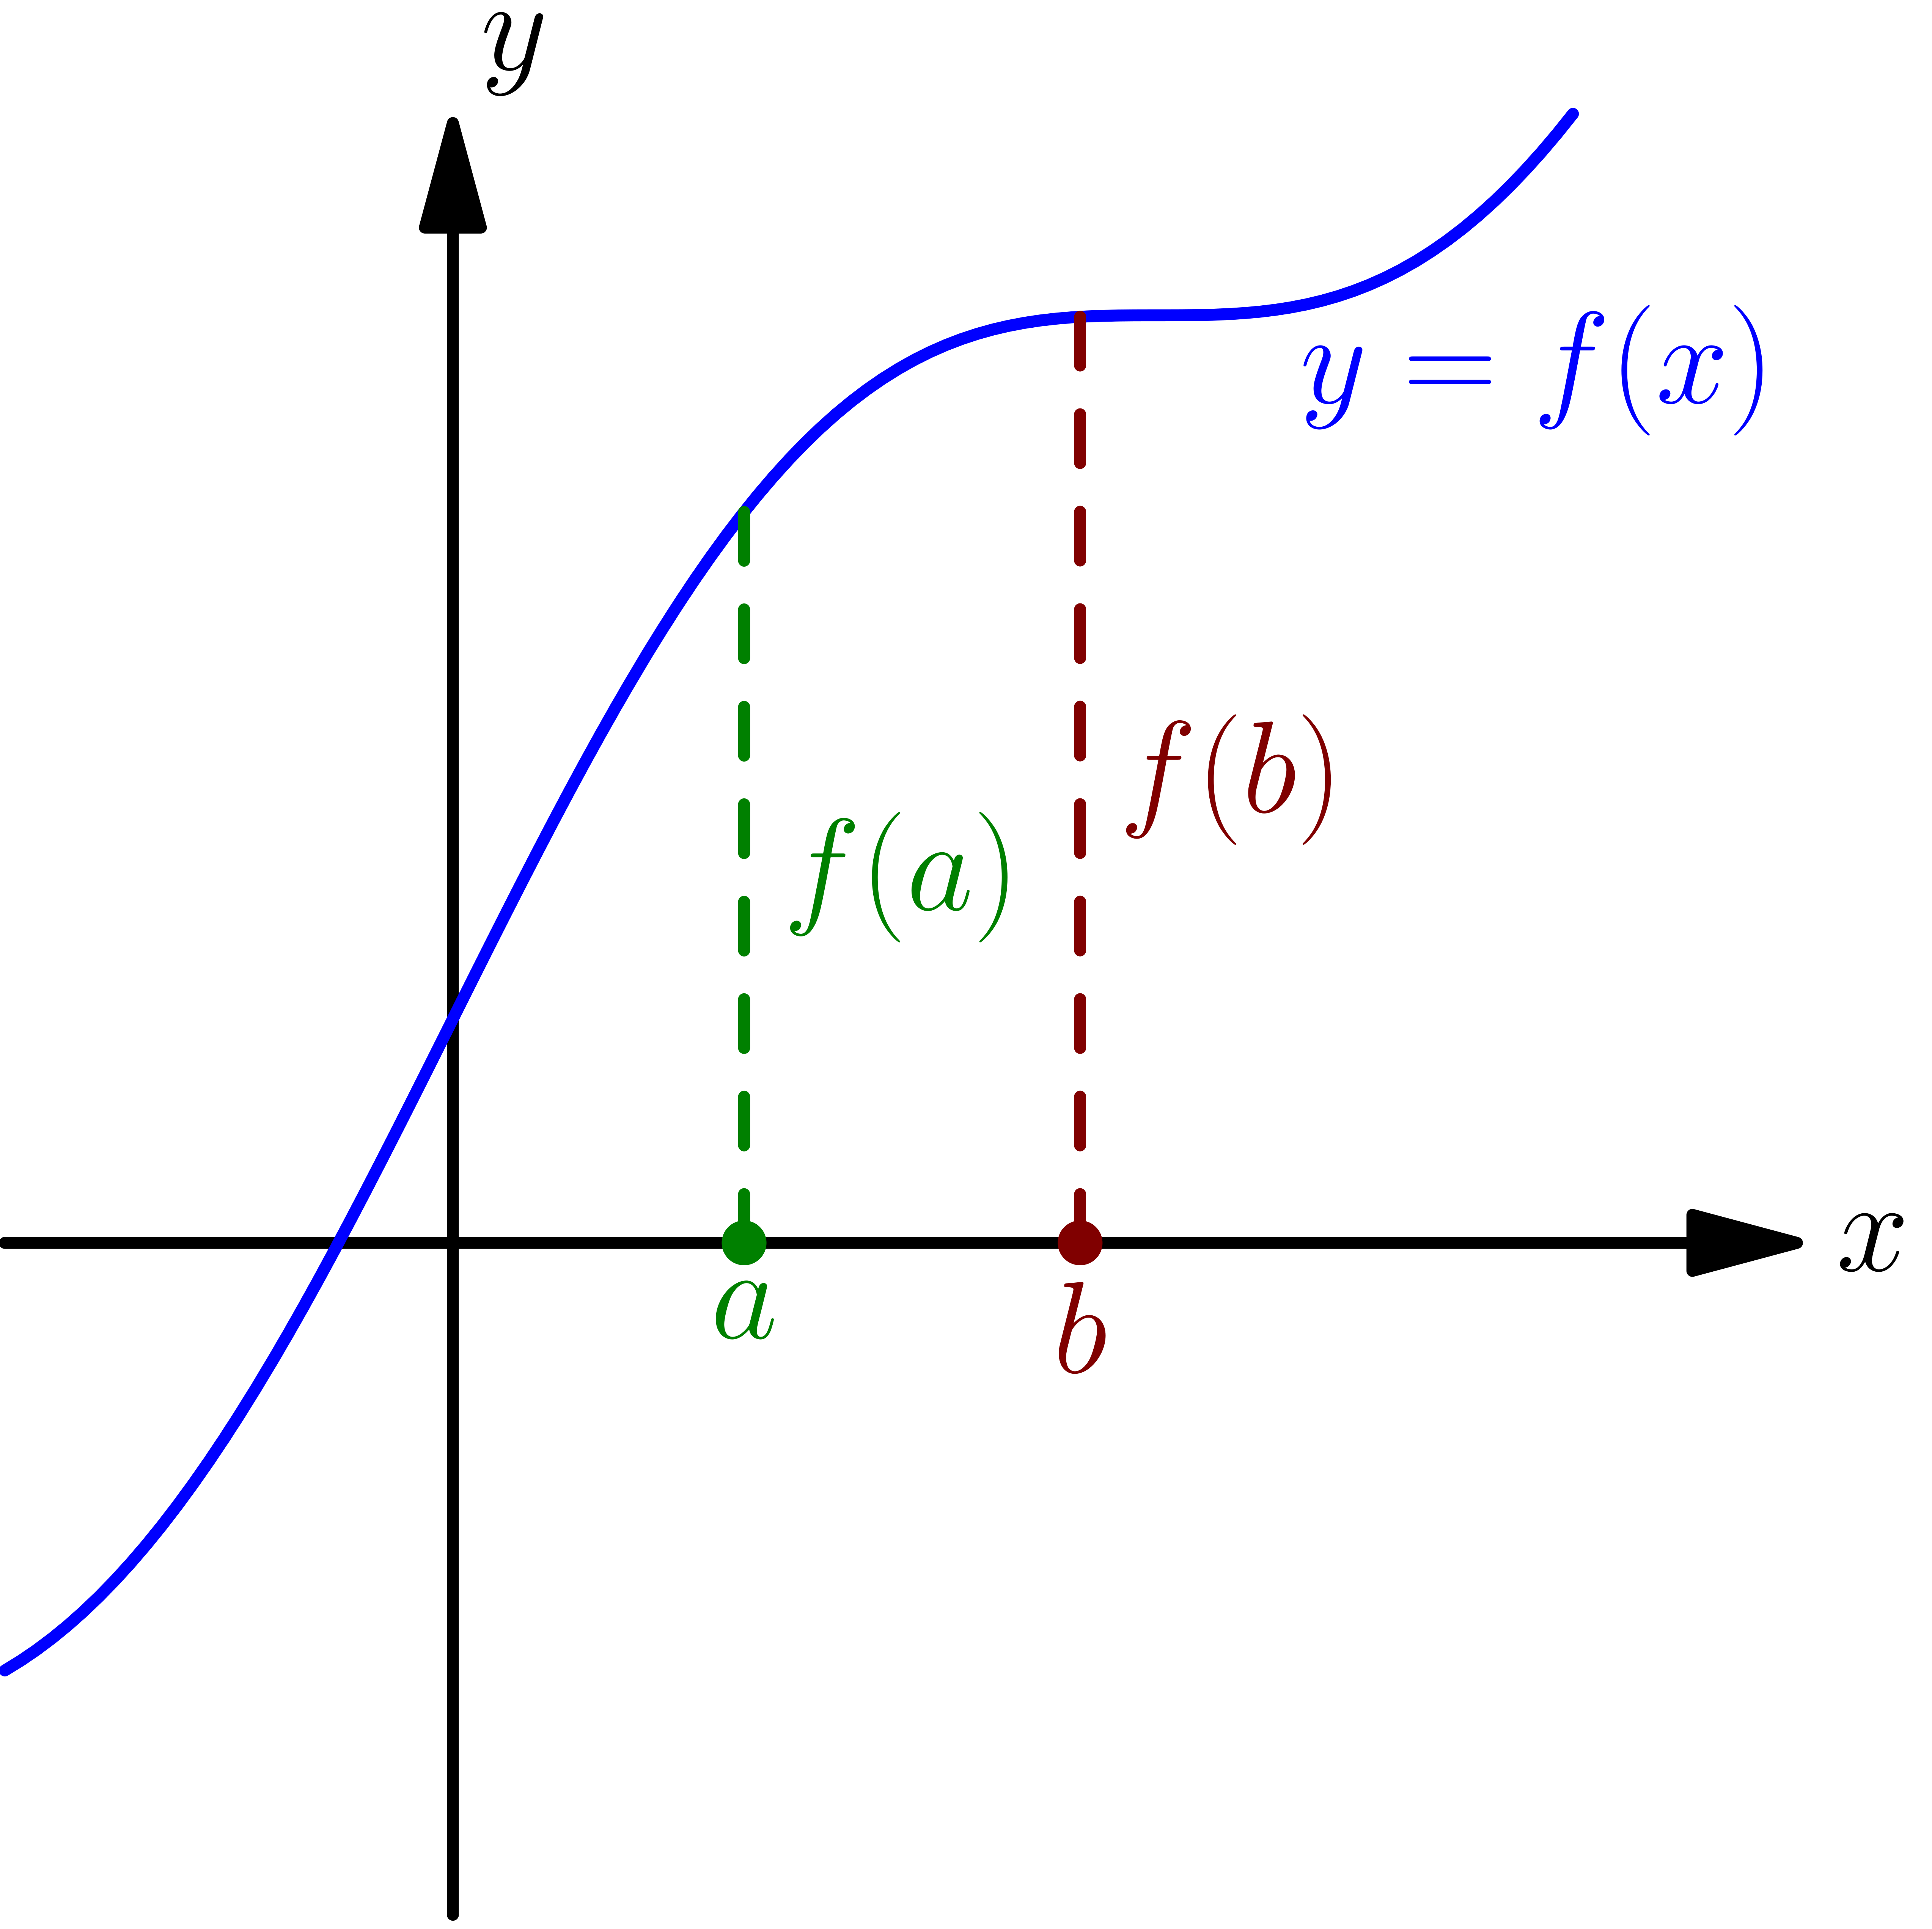
\includegraphics[width=0.4\linewidth]{chapters/chapter 5/increasing.png} }}%
    \qquad
    \subfloat{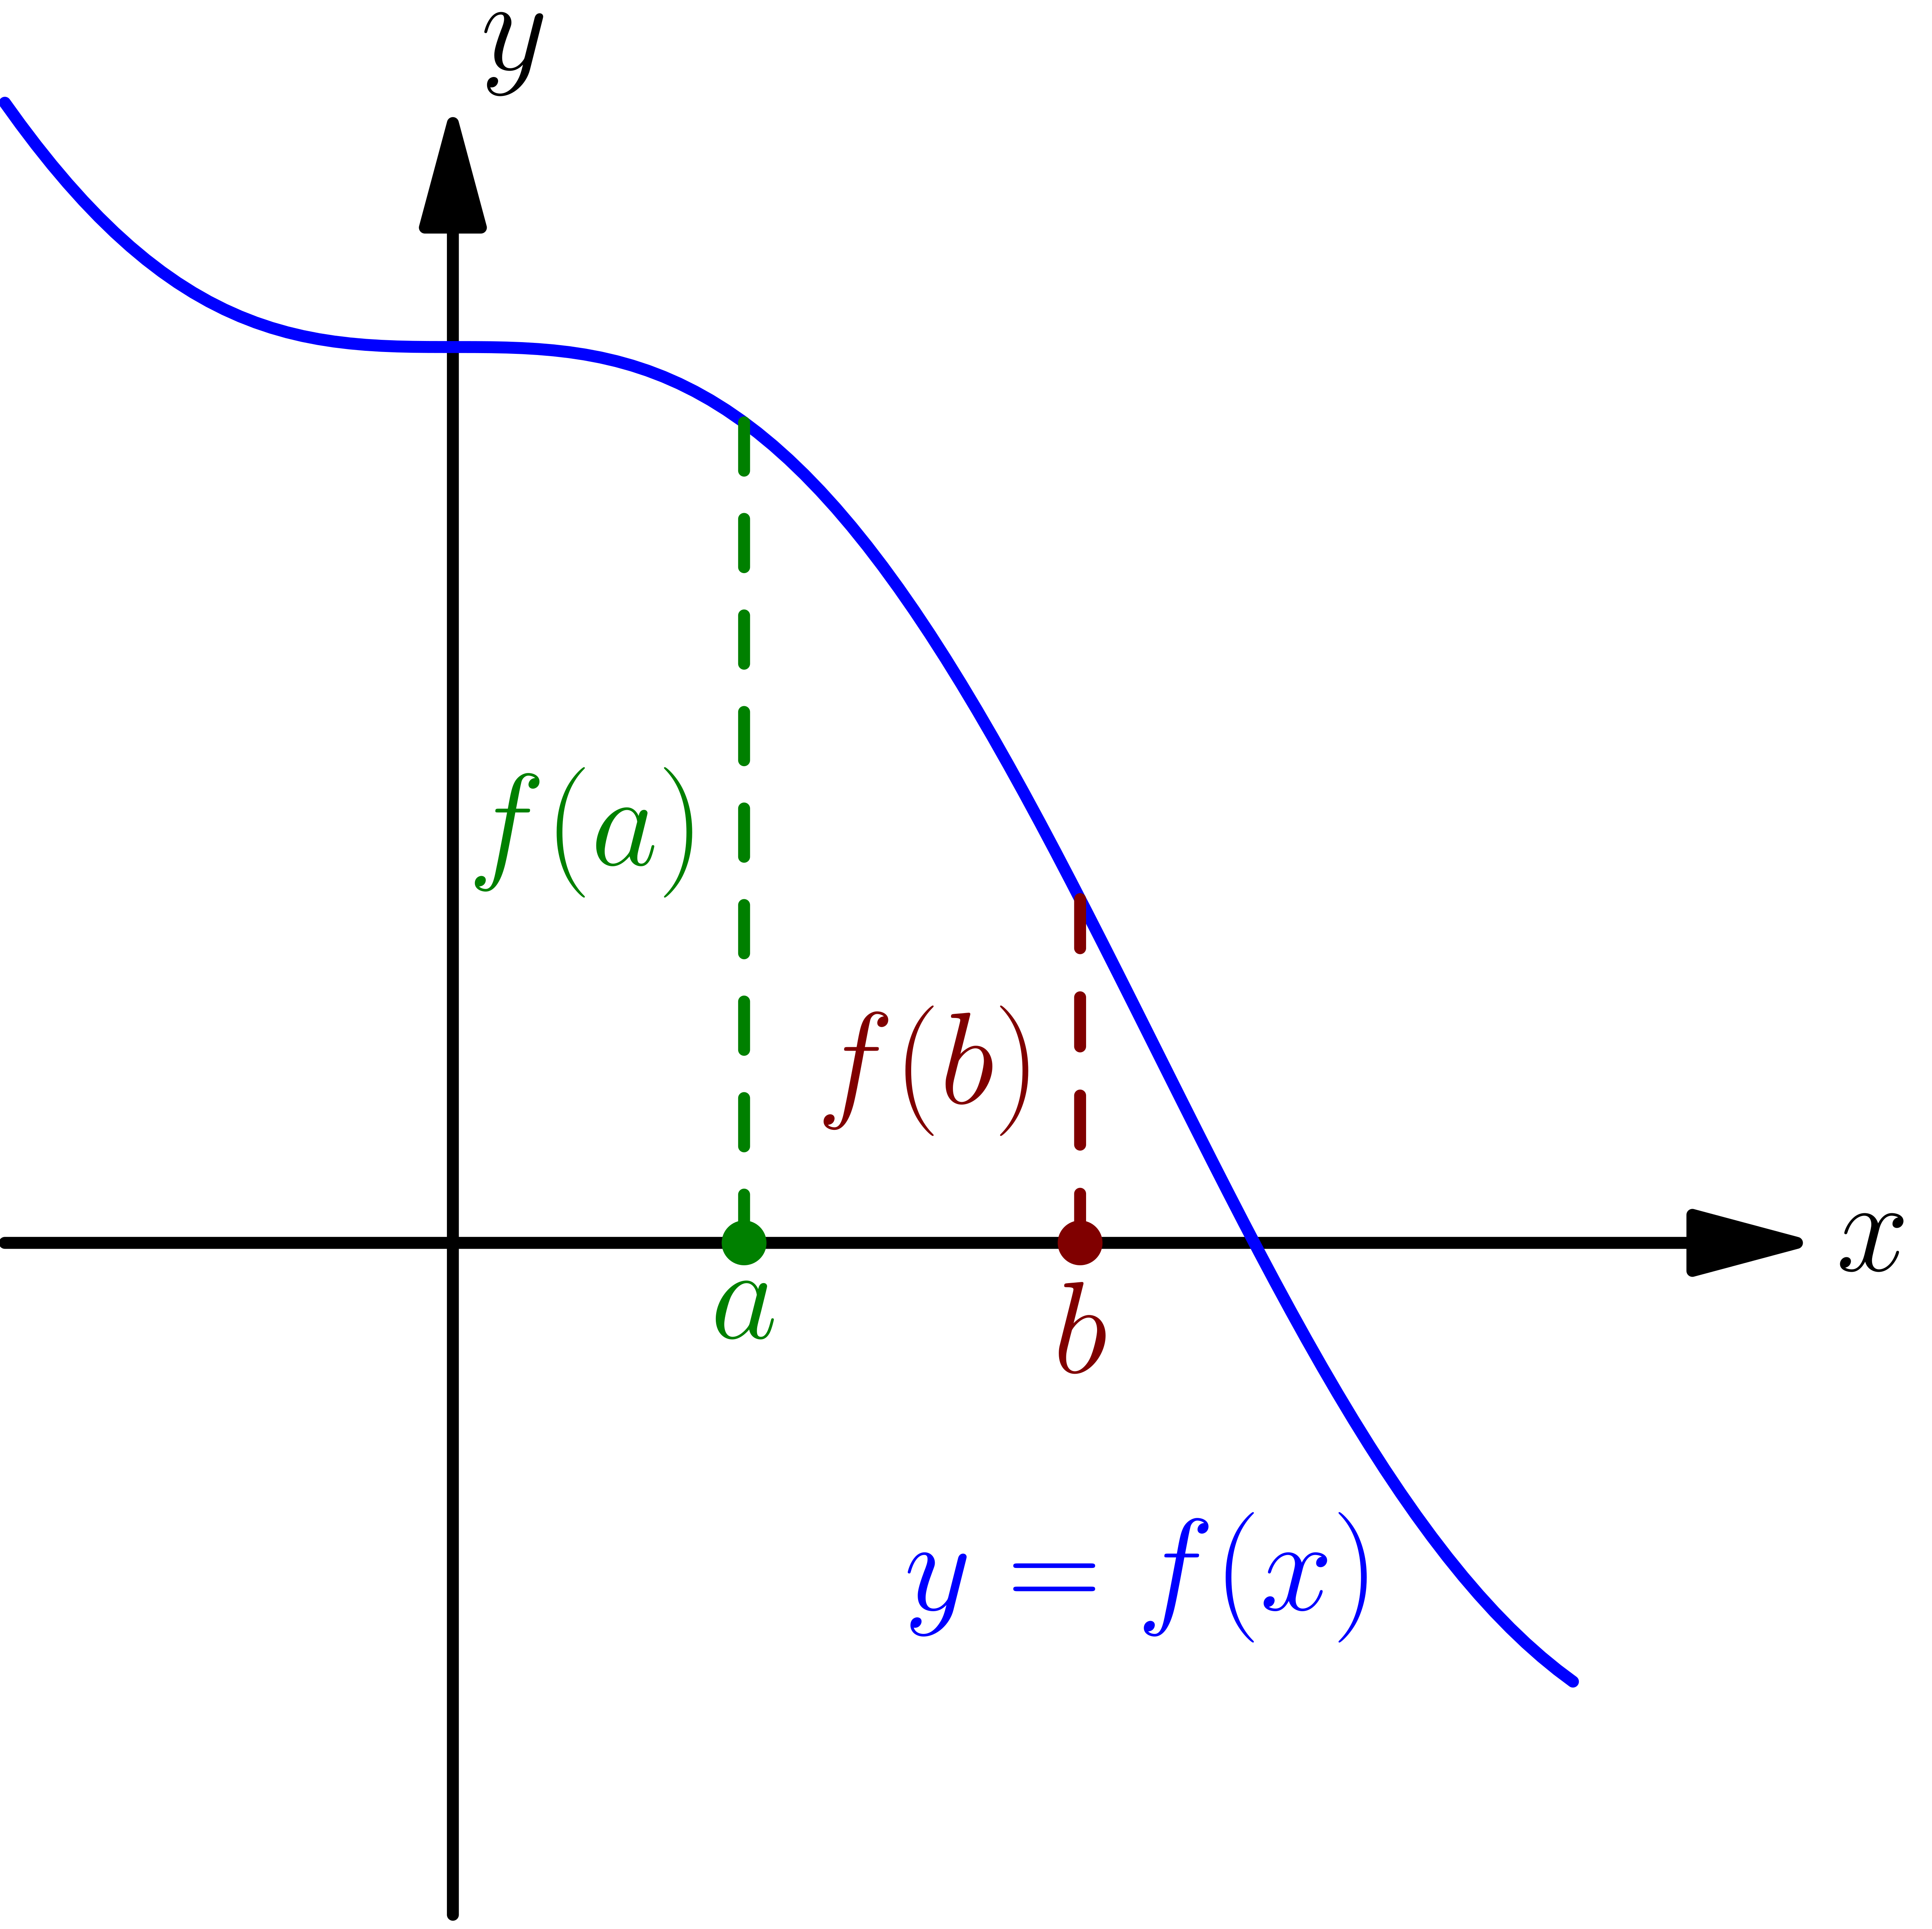
\includegraphics[width=0.4\linewidth]{chapters/chapter 5/decreasing.png}} %
    % \caption*{աճողը և նվազողը}
\end{figure}

Նման ձևով կարող ենք սահմանել նաև \textit{չնվազող՝}
\[f(c) \le f(a) \le f(b) \qquad \text{եթե } c<a<b\]
և \textit{չաճող՝}
\[f(c) \ge f(a) \ge f(b) \qquad \text{եթե } c<a<b\]
ֆունկցիայի գաղափարները, որոնք ներառում են նաև հավասարության դեպքերը։

\question{Կարո՞ղ եք գծել/գրել այնպիսի ֆունկցիա, որը $0$-ում աճող է, $1$-ում՝ նվազող: Ո՞ր ֆունկցիան է և՛ չաճող, և՛ չնվազող։}

Յուրաքանչյուր կետում կարող ենք պարզել՝ ֆունկցիան աճում է, թե նվազում, նայելով միայն նրա ածանցյալի նշանին։\marginnote[*+3]{դրական արագություն $=$ աճող\\բացասական արագություն $=$ նվազող}

\begin{theorem}
Ենթադրենք $f$ ֆունկցիան դիֆերենցելի է $a$ կետում։ Ուրեմն
\begin{itemize}
    \item եթե $f'(a) > 0$, ապա $f$-ն $a$-ում աճող է
    \item եթե $f'(a) < 0$, ապա $f$-ն $a$-ում նվազող է
    \item եթե $f'(a) \ge 0$, ապա $f$-ն $a$-ում չնվազող է
    \item եթե $f'(a) \le 0$, ապա $f$-ն $a$-ում չաճող է
\end{itemize}
\end{theorem}

\question{Ներքևում բերված ֆունկցիայի ածանցյալը ո՞ր կետերում է դրական։ Իսկ որոնցո՞ւմ է բացասական։}

\begin{figure}[h]
    \centering
    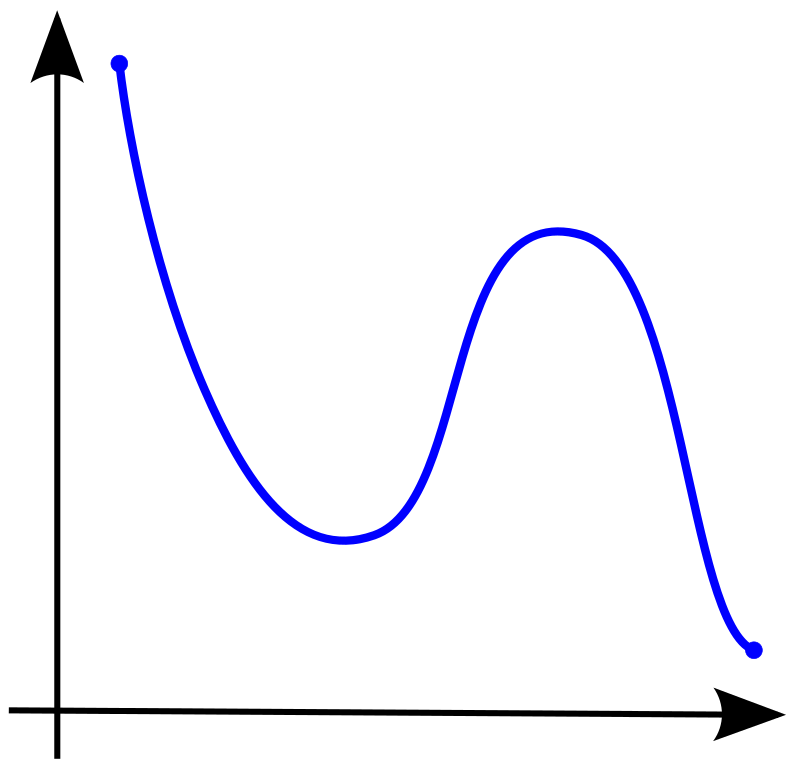
\includegraphics[width=0.4\linewidth]{chapters/chapter 5/just another function.png}
\end{figure}

\question{Պատկերացրեք՝ \hyperref[apricot]{\color{OliveGreen}ծիրանի գինը} դրել եք $x=4$։ Կմեծանա՞, թե՞ կփոքրանա խանութի եկամուտը, եթե գինը մի փոքր բարձրացնեք։}

\section{Էքստրեմումի խնդրի լուծումը}\label{single_var_extrema}

Փաստորեն արդեն գիտենք, թե ինչպես ածանցյալի նշանից հասկանալ՝ գինը բարձրացնե՞լ, թե՞ իջեցնել՝ եկամուտը մեծացնելու համար։ Իսկ ինչպե՞ս պարզել, թե որ գնի դեպքում է եկամուտն ամենամեծը, այլ կերպ ասած՝ ո՞ր $x$ կետում է ֆունկցիան ընդունում իր ամենամեծ արժեքը։ 

\question{Ենթադրենք $f$ ֆունկցիան իր ամենամեծ արժեքը ընդունում է $a$ կետում։ Ի՞նչ կարող եք ասել այդ կետում $f$-ի ածանցյալի մասին։}

\marginnote[*+1]{իսկ այն կետը, որում ֆունկցիան ընդու\-նում է այդ արժեքը, կանվանենք գլո\-բալ մաքսիմումի/մինիմումի \textit{կետ}}Պայմանավորվենք ֆունկցիայի ընդունած ամենամեծ արժեքն անվանել ֆունկցիայի \textit{գլոբալ մաքսիմում,} ամենափոքրը՝ \textit{գլոբալ մինիմում,} իսկ այս երկուսը միասին՝ \textit{գլոբալ էքստրեմումներ։} 

\warning{Որոշ ֆունկցիաներ ունեն գլոբալ մաքսիմում, որոշ ֆունկցիաներ՝ ոչ։}

\begin{example}\label{extrema_example}
Գծելով հետևյալ ֆունկցիաների գրաֆիկները՝ կնկատեք, որ
\begin{itemize}
    \item $f(x)=x^2$ ֆունկցիան ունի 
    \begin{itemize}
        \item[-] գլոբալ մինիմում $x=0$ կետում
        \item[-] գլոբալ մաքսիմում չունի
    \end{itemize}
    
    \item $f(x)=-x^2$ ֆունկցիան ունի
    \begin{itemize}
        \item[-] գլոբալ մաքսիմում $x=0$ կետում
        \item[-] գլոբալ մինիմում չունի    \marginnote{այստեղ կարող էին լինել գրաֆիկներ, բայց փոխարենը կա \href{https://www.desmos.com}{հղում}}
    \end{itemize}
    
    \item $f(x)=25x^4 - 50x^2 + 16$ ֆունկցիան ունի
    \begin{itemize}
        \item[-] գլոբալ մինիմում $x=-1$ և $x=1$ կետերում
        \item[-] գլոբալ մաքսիմում չունի
    \end{itemize}
        
    \item $f(x)=\dfrac{\sin{x}}{x}$ ֆունկցիան ունի
    \begin{itemize}
        \item[-] գլոբալ մինիմում $x \approx -4.49$ և $x \approx 4.49$ կետերում
        \item[-] գլոբալ մաքսիմում $x=0$ կետում
    \end{itemize}
    
    % \item $f(x)=\cos{x}$ ֆունկցիան ունի 
    % \begin{itemize}
    %     \item[] գլոբալ մինիմում $x \approx -4.49$ և $x \approx 4.49$ կետերում
    %     \item[] գլոբալ մաքսիմում $x=0$ կետում
    % \end{itemize}
    
    % գլոբալ մինիմում $x = \pm\pi, \pm3\pi, \pm5\pi, \dots$ կետերում, իսկ գլոբալ մաքսիմում՝ $x=0, \pm2\pi, \pm4\pi, \dots$ կետերում
    \item $f(x)=5$ ֆունկցիան միշտ ընդունում է նույն արժեքը, որը և՛ գլոբալ մաքսիմումն է, և՛ գլոբալ մինիմումը
    
    \item $f(x)=3x+1$ ֆունկցիան չունի ոչ գլոբալ մաքսիմում, ոչ գլոբալ մինիմում
\end{itemize}

Ի՞նչ կարող եք ասել $f(x)=\cos x$-ի գլոբալ էքստրեմումների մասին։
\end{example}

Իսկ ինչո՞ւ ենք շեշտում «գլոբալ», մի՞թե կան այլ մինիմումներ։ Հիշենք նախորդ բաժնում պատկերված \hyperref[local_extr]{\color{OliveGreen}այս} ֆունկցիան։ Քանի որ այն աջ գնալիս շարունակ փոքրանում է՝ ընդունելով ավելի ու ավելի փոքր արժեքներ, ապա այն գլոբալ մինիմում չունի։ Սակայն նկատենք, որ $x\approx -2$ կետի մոտակայքում ֆունկցիան մի պահ նվազելով իջնում է ներքև, ապա սկսում դանդաղ բարձրանալ վերև, ինչի արդյունքում առաջանում է մի փոքր փոսիկ։ 

\begin{marginfigure}
    \centering
    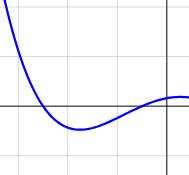
\includegraphics[width=0.6\linewidth]{chapters/chapter 5/zoomed function.png}
    \caption*{կամ այնքան մոտեցնենք ({\rm zoom} անենք), որ միայն այդքան մասը երևա}
\end{marginfigure} Հենց այդ փոսիկը կոչվում է ֆունկցիայի \textit{լոկալ մինիմում՝} այն իմաստով, որ եթե ֆունկցիան կտրենք, ասենք, $-3$ և $-1$ կետերի միջև ու նայենք ստացված փոքր տեղամասին, ապա կունենանք լոկալ մասշտաբով ամենափոքր արժեք։ Նույն ձևով՝ $x \approx 0.5$ կետի մոտակայքում ունենք «փոքրիկ» լոկալ մաքսիմում։ 

Ավելի պատկերավոր՝ Ջոմոլունգման գլոբալ մաքսիմում է, Մասիս սարը՝ լոկալ մաքսիմում։ Գլոբալ մաքսիմումն, իհարկե, կարևոր է, բայց ինչպես կտեսնենք, լոկալ մաքսիմումները նույնպես չարժի աչքաթող անել։

\begin{definition}
Կասենք, որ $f$-ը $a$ կետում ընդունում է \textbf{լոկալ մաքսիմում} (մինիմում), եթե բավականաչափ փոքր $(a-\delta, a+\delta)$ միջակայքի կետերում $f$-ի ամենամեծ (ամենափոքր) արժեքը $f(a)$-ն է։
\end{definition}

Կամ այլ կերպ ասած՝ եթե գոյություն ունի այնպիսի $\delta > 0$ թիվ, որ եթե $a - \delta < x < a + \delta$, ապա $f(x) \le f(a)$ (լոկալ մինիմումի դեպքում՝ $\ge$):

\begin{figure}[t]
    \centering
    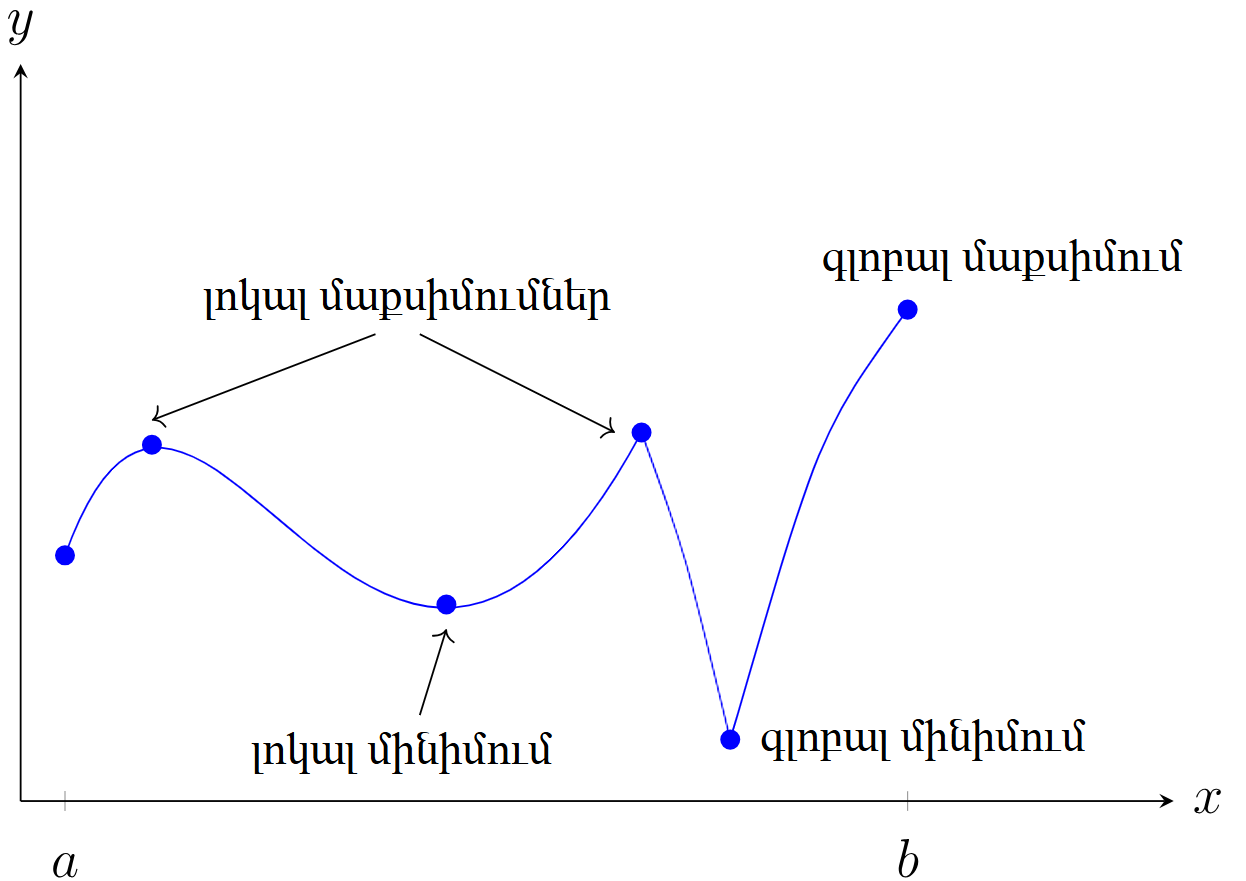
\includegraphics[width=0.65\linewidth]{chapters/chapter 5/extrema.png}
\end{figure}

\question{Որո՞նք են \hyperref[extrema_example]{\color{OliveGreen}նախորդ օրինակի} ֆունկցիաների լոկալ էքստրե\-մում\-ները (եթե իհարկե կան)։}

Բնականաբար, ամեն մի գլոբալ էքստրեմում նաև լոկալ էքստրեմում է, իսկ այ հակառակը՝ ոչ միշտ է ճիշտ։ Վերևում տեսել ենք, որ հնարա\-վոր է՝ ֆունկցիան ընդհանրապես չունենա գլոբալ կամ նույնիսկ լոկալ մաքսիմում/մինիմում (քանի որ, օրինակ, միշտ ավելի ու ավելի մեծ/փոքր արժեքներ է ընդունում)։ Նշենք միայն, որ եթե $x$-երը սահմանա\-փակենք ինչ-որ մի փակ (այսինքն՝ $[a, b]$ տեսքի)\marginnote{փակ $=$ ծայրակետերը ներառյալ} միջակայքում, ապա երաշխավորված է, որ այդքան տեղում կունենանք և՛ գլոբալ մինիմում, և՛ գլոբալ մաքսիմում․

\begin{theorem}
Եթե $f$-ն անընդհատ ֆունկցիա է, ապա այն ցանկա\-ցած $[a, b]$ միջակայքում ունի գլոբալ մաքսիմում և մինիմում։
\end{theorem}

Վերջապես ինչպե՞ս գտնենք ֆունկցիայի լոկալ կամ գլոբալ էքստրեմում\-ները։ Պատասխանը կրկին թաքնված է ֆունկցիայի ածանցյալի նշանի մեջ։ Ենթադրենք՝ ինչ-որ $a$ կետում $f$ ֆունկցիան ընդունում է լոկալ մինիմումի արժեք, այսինքն՝ լոկալ իմաստով $a$-ի շրջակայքում $f(a)$-ից փոքր արժեք չկա։ Լավ, ուրեմն կարո՞ղ է $a$ կետում $f$-ի ածանցյալը լինել բացասական։ 

\newpage

Եթե այն բացասական լինի, ապա $f$-ը $a$-ում պետք է լինի նվազող, այսինքն՝ մի փոքր առաջ գնալով ($a$-ից աջ՝ ինչ-որ մի $a+\delta$ կետում) ֆունկցիայի արժեքը կլինի ավելի փոքր, քան $a$-ում։ Ինչը, սակայն, բացառված է, քանի որ $a$-ն լոկալ մինիմումի կետ է․ նշանակում է $f'(a)$-ն բացասական չէ՝ $f'(a) \ge 0$: 

\question{Կարո՞ղ է $f'(a)$-ն լինել դրական։}

Ենթադրելով, որ հարցին պատասխանեցիք «ոչ» և նմանատիպ ձևով ապացուցեցիք դա, ֆիքսենք՝ $f'(a) \le 0$: Ուրեմն միակ հնարավոր տարբերակը մնաց՝ կա՛մ $f$-ը $a$ կետում ընդհանրապես ածանցյալ չունի, կա՛մ էլ եթե ունի, ապա $f'(a) = 0$։ Այդպիսի կետերին անվանում ենք \textit{կրիտիկական կետեր։}

\begin{theorem}
\marginnote{այսինքն՝ եթե կա $f'(a)$, ապա $f'(a)=0$}Եթե $a$-ն $f$-ի լոկալ կամ գլոբալ էքստրեմումի կետ է, ապա այն կրիտիկական կետ է։
\end{theorem}

\warning{Կրիտիկական կետ լինելը դեռ չի նշանակում, որ կետը էքստրեմումի կետ է։}

\begin{example}
Գծենք հետևյալ երեք ֆունկցիաների գրաֆիկները․
\begin{itemize}
\item $f_1(x)=x^2$, որի համար $x=0$-ն մինիմումի կետ է։ Իրոք՝
\[ f_1'(x)=2x,\qquad f_1'(0)=0 \]

\item $f_2(x)=-x^2$, որի համար $x=0$-ն մաքսիմումի կետ է՝
\[ f_2'(x)=-2x,\qquad f_2'(0)=0 \]

\item $f_3(x)=x^3$, որի համար $x=0$-ն ոչ մինիմումի, ոչ մաքսիմումի կետ է, մինչդեռ՝
\[ f_3'(x)=3x^2,\qquad f_3'(0)=0 \]
\end{itemize}
\end{example}

Փաստորեն $f'(x)=0$ պայմանը անհրաժեշտ է, բայց \textit{բավարար չէ․} ամեն կրիտիկական կետ չէ, որ լոկալ էքստրեմումի կետ է։ Երրորդ ֆունկցիայի դեպքում, օրինակ, ածանցյալի զրո լինելը նշանակում էր՝ ֆունկցիան աճելով եկավ, արագությունը նվազեցրեց, դարձրեց $0$, բայց հետո նորից սկսեց մեծացնել ու շարունակեց աճել (այլ ոչ թե սկսեց նվազել)։

Լավ, բա ի՞նչ անենք։ Պատկերացրեք՝ կրկին գրաֆիկը նստած իջնում եք դեպի ֆունկցիայի լոկալ մինիմումի կետը։ Քանի դեռ չեք հասել այդ կետին, արագությունը բացասական է (կամ առնվազն՝ ոչ դրական), որովհետև իջնում եք։ Հասնելով այդ կետին՝ արագությունը դառնում է $0$ (կրիտիկական կետ է)։ Ի՞նչ է լինում, երբ այդ կետը անցնում ու գնում եք առաջ։ Քանի որ լոկալ մինիմումի կետն անցել եք, ապա ֆունկցիայի գրաֆիկը պետք է բարձրանա․ արագությունը ոչ բացասական է։ Ուրեմն՝

\newpage


\begin{theorem}
\begin{marginfigure}
    \centering
    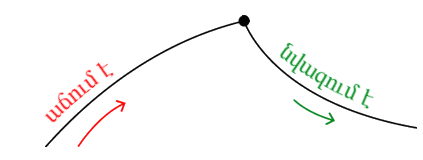
\includegraphics[width=0.8\linewidth]{chapters/chapter 5/derivative test.png}
\end{marginfigure}Եթե $f$-ը դիֆերենցելի է $a$ կետի մի որևէ $(a-\delta, a+\delta)$ շրջակայքում,
\begin{itemize}
    \item \item եթե $a$ կետից ձախ $f'(x) > 0$, իսկ $a$-ից աջ՝ $f'(x) < 0$, ապա $a$-ն լոկալ մաքսիմումի կետ է
    \item եթե $a$ կետից ձախ $f'(x) < 0$, իսկ $a$-ից աջ՝ $f'(x) > 0$, ապա $a$-ն լոկալ մինիմումի կետ է
    \item եթե $a$ կետից աջ և ձախ $f'(x)$-ի նշանը նույնն է, ապա $a$-ն լոկալ էքստրեմումի կետ չէ
\end{itemize}
\end{theorem}

\question{Ինչպե՞ս կարտահայտեք $f'$-ի նշանի՝ դրականից բացասական դառնալը՝ օգտվելով $f''$-ից։}

Այն դեպքում, երբ հարմար չէ հաշվել $f'$-ը/հետազոտել դրա նշանը, բայց փոխարենը հեշտ է գտնել $f$-ի երկրորդ կարգի ածանցյալը, կարող ենք օգտվել հետևյալ թեորեմից․

\begin{theorem}
Եթե $f'(a)=0$ և
\begin{itemize}
    \item $f''(a) > 0$, ապա $a$-ն լոկալ մինիմումի կետ է
    \item $f''(a) < 0$, ապա $a$-ն լոկալ մաքսիմումի կետ է
\end{itemize}
\end{theorem}

Ուշադրություն դարձնենք, որ թեորեմը չի պատասխանում այն հարցին, թե ինչ է տեղի ունենում, երբ $f''(a)=0$: Այդ դեպքում այս թեորեմն անօգուտ է, բայց կարելի է օգտվել նախորդ թեորեմից։


\bigskip 

\begin{theory}
.
\begin{itemize}
\item կարդալ [{\rm Stewart}], 87-91 (սահման), 118-121 (անընդհատու\-թյուն), 146-148, 154-161 և 199-201 (ածանցյալ), 274-279 (էքստրեմումներ) էջերը  
\item ըստ ցանկության՝ [{\rm Stewart}], 99-101, 174-180, 184-189, 290-292 էջերը
\item դիտել  {\rm 3b1b}-ի \href{https://www.3blue1brown.com/lessons/essence-of-calculus}{1-ին}, \href{https://www.3blue1brown.com/lessons/derivatives}{2-րդ} և \href{https://www.3blue1brown.com/lessons/limits}{8-րդ} տեսադասերը մաթանալիզից 
\item ըստ ցանկության՝ նաև \href{https://www.3blue1brown.com/lessons/epsilon-delta}{9-րդը}
\item կարելի է նաև գտնել լուծված վարժություններ \href{https://tutorial.math.lamar.edu/Classes/CalcI/CalcI.aspx}{այստեղ}
\end{itemize}
\end{theory}

\newpage

\section{Խնդիրներ}

\begin{problem}
Ունի՞ արդյոք հաջորդականությունը սահման (երբ $n\to\infty$)։ Եթե այո, ապա գտեք այն․

\begin{enumerate}[label={\alph*}․]
\item $\dfrac{3-n}{2}$

\item $\dfrac{4\sqrt{n}}{n^3}$

\item $\dfrac{n-1}{n^2-1}$

\item $1^n$

\item $0.4^n$

\item $(-4)^n$

\item որպես առաջին անդամ՝ վերցրեք ցանկացած թիվ, \\որպես երկրորդ անդամ՝ վերցրեք առաջինը բաժանած $1.5$-ի, \\ապա՝ երկրորդը բաժանած $1.5$-ի, և այդպես շարունակ

\item $a_1=1$, \\$a_2 = \dfrac{a_1}{7}$-ում ստորակետից հետո գրված առաջին թվանշանը, \\$a_3= \dfrac{a_2}{7}$-ում ստորակետից հետո գրված առաջին թվանշանը,
\\$\dots$

\end{enumerate}

\hint{Որպեսզի զգաք, թե ինչպես է փոխվում հաջորդականու\-թյու\-նը, գրեք դրա առաջին մի քանի անդամները։ Վերջին կետում օգտվեք հաշվիչից։}
\end{problem}


\begin{problem}
Սահմանների մասին \hyperref[limit_properties]{\color{OliveGreen}թեորեմում} ոչինչ չէինք կարող ասել $\dfrac{a_n}{b_n}$-ի սահմանի մասին, երբ $\lim\limits_{n\to\infty} b_n = 0$։ Կարո՞ղ եք բերել այնպիսի $a$ և $b$ հաջորդականությունների օրինակներ, որոնց համար $\lim\limits_{n\to\infty} a_n = 0$, $\lim\limits_{n\to\infty} b_n = 0$, բայց
\begin{enumerate}[label={\alph*}․]
\item $\lim\limits_{n\to\infty} \dfrac{a_n}{b_n} = 1$

\item $\lim\limits_{n\to\infty} \dfrac{a_n}{b_n} = -5$

\item $\lim\limits_{n\to\infty} \dfrac{a_n}{b_n} = 0$

\item $\lim\limits_{n\to\infty} \dfrac{a_n}{b_n} = +\infty$

\item $\lim\limits_{n\to\infty} \dfrac{a_n}{b_n}$ գոյություն չունի
\end{enumerate}
\end{problem}


\begin{problem}
Հետևյալ ֆունկցիաները բաղկացած են $x=2$ կետում իրար «սոսնձած» երկու առանձին ֆունկցիաներից։ Կարո՞ղ եք գտնել $c$-ի այնպիսի արժեք, որի դեպքում ֆունկցիան անընդհատ լինի $2$-ում։\marginnote[*+2.5]{\href{https://www.desmos.com/calculator/c3047befa7}{սկզբից փորձեք աչքաչափով}}

\begin{enumerate}[label={\alph*}․]
\item \marginnote[*+2]{\href{https://www.desmos.com/calculator/8eb756f334}{սա նույնպես}} $f(x)=\begin{cases} 3x-5& \text{եթե }x<2 \\  x^2+c& \text{եթե }x \ge 2 \end{cases}$

\item $
f(x)=\begin{cases} x^3+1& \text{եթե } x<2 \\  cx^2& \text{եթե } x \ge 2 \end{cases} $ 

\item $
f(x)=\begin{cases} -7& \text{եթե } x<2 \\ c& \text{եթե } x=2 \\  4+3\sin(\pi x)& \text{եթե } x>2 \end{cases} $
\bigskip

\item $
f(x)=\begin{cases} {\dfrac{x^2-x-2}{x-2}}& \text{եթե }x \ge 2 \\  c& \text{եթե }x<2 \end{cases} $

\end{enumerate}
\end{problem}


\begin{problem}
Զևսը, Պրոմեթևսն ու Արամազդը $1000$-ական ոսկի են ավանդ դնում համապատասխանաբար
\begin{enumerate}
    \item ՕլիմպոսԲանկում, որտեղ գումարը $x$ տարի հետո կազմելու է $f(x)=100x+x^3$ ոսկի
    \item ՏավրոսԲանկում, որտեղ գումարը $x$ տարի հետո կազմելու է $f(x)=0.18x^3\cdot \sqrt{x}$ ոսկի
    \item ԱրարատԲանկում, որտեղ գումարը $x$ տարի հետո կազմելու է $f(x)=30x^2$ ոսկի
\end{enumerate}

Հաշվի առնելով, որ երեքն էլ անմահ են, նրանցից ո՞վ ի վերջո ավելի հարուստ կլինի $\infty$ շատ ժամանակ անց։
\end{problem}

\begin{problem}
Գտեք հետևյալ ֆունկցիաների ածանցյալները․
\begin{enumerate}[label={\alph*}․]
\item $f(x)=10000$
\item $f(x)=2x^2-7x+1$
\item $f(x)=2\sin x \cdot e^x$
\item $f(x)=e^{x^2}$
\item $f(x)=x^2\ln x$
\item $f(x)=\dfrac{x^2}{x^3}$\marginnote[*+1.5]{\href{https://youtu.be/ejtfAp_7PD8}{լուծում}}
\item $f(x)=\sin(\cos x)$
\item $f(x)=x^x$
\end{enumerate}
\end{problem}

\begin{problem}
Մեքենայական ուսուցման մեջ հաճախ օգտագործվում են հետևյալ երկու ֆունկցիաները.
\begin{enumerate}[label={\alph*}․]
\item {\rm ReLU (rectified linear unit)}՝
\\ $f(x) = \begin{cases}
    x & \text{եթե } x>0\\
    0 & \text{եթե } x\le 0
\end{cases}$

\begin{center}
\begin{tikzpicture}[scale=0.5]
\begin{axis}[
    axis lines = middle,
    xlabel = {$x$},
    ylabel = {$f(x)$},
    domain = -2:2,
    samples = 100,
    ymin = -1,
    ymax = 2,
    width=0.8\textwidth
]
\addplot[color=blue, thick] {max(0,x)};
\end{axis}
\end{tikzpicture}
\end{center}

\item Սիգմոիդ՝
\\ $f(x) = \dfrac{1}{1+e^{-x}}$

\begin{center}
\begin{tikzpicture}[scale=0.5]
\begin{axis}[
    axis lines = middle,
    xlabel = {$x$},
    ylabel = {$f(x)$},
    domain = -6:6,
    samples = 100,
    ymin = -1,
    ymax = 2,
    width=0.8\textwidth
]
\addplot[color=blue, thick] {1 / (1 + exp(-x))};
\end{axis}
\end{tikzpicture}
\end{center}

\end{enumerate}

Հաշվեք դրանց ածանցյալները։ Կարո՞ղ եք սիգմոիդի ածանցյալն արտահայտել սիգմոիդով։
    
\end{problem}


\begin{problem}\marginnote[*+0.5]{\href{https://youtu.be/BnhCUCzmWeM}{լուծում}}
Դիցուք ունենք որևէ $\R^2 \to \R^2$ գծային ձևափոխություն՝
\[
A = \begin{bmatrix}
    a & b \\ c & d
\end{bmatrix}
\]
և ցանկանում ենք պարզել՝ ինչ տեղի կունենա, եթե այն մի փոքր փոփոխենք (օրինակ՝ $A + 0.001 \cdot I$)։ Մասնավորապես՝ որքա՞ն կփոխվի ձևափոխության որոշիչը, եթե նրան գումարենք (փոքր թիվ) $\times$ (միավոր մատրից)։

Դա պարզելու համար համար նշանակենք՝
\[
f(x) = \det(A+x \cdot I)
\]

\begin{enumerate}[label={\alph*}․]
\item ինչի՞ է հավասար $f(0)$-ն
\item օգտվելով ածանցյալի բանաձևից՝ գտեք $f'(0)$-ն
\item ճանաչեցի՞ք
\end{enumerate}
\end{problem}


\begin{problem}
Գտեք հետևյալ ֆունկցիաների լոկալ մինիմումի և մաքսի\-մու\-մի կետերը (եթե կան)․
\begin{enumerate}[label={\alph*}․]
\item $f(x)=5x-x^2$
\item $f(x)=3x+1$
\item $f(x)=\dfrac{x^3}{e^x}$
\end{enumerate}
\end{problem}

\begin{problem}\marginnote[*+0.5]{\href{https://youtu.be/f2Bp77tiESg}{լուծում}}
Ունենք  $24$ մ$^2$ մակերեսով ստվարաթուղթ (ինչպես նաև մկրատ ու սոսինձ), որով ցանկանում ենք պատրաստել այսպիսի տուփ՝
\begin{figure}[h]
    \centering
    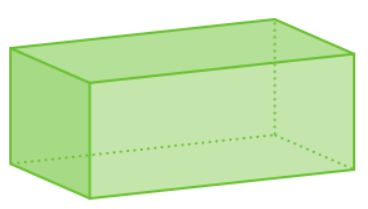
\includegraphics[width=0.4\linewidth]{chapters/chapter 5/top-ov-box.png}
\end{figure}

որի ձախ և աջ նիստերը քառակուսիներ են։ 

Ամենաշատը որքա՞ն կարող է լինել այդ տուփի ծավալը։ 

\hint{Նախ՝ մի քիչ երկրաչափություն։ Վերցրեք ոչ քառակուսի նիստերից մեկը, նշանակեք դրա երկարությունն ու լայնությունը $x$ և $y$։ Կարո՞ղ եք $y$-ն արտահայտել $x$-ով։ Իսկ ծավալը՝ $x$-ո՞վ։}
\end{problem}